\documentclass[twocolumn, 11pt]{article}
\usepackage{amsmath,amssymb}
\usepackage[format=hang,labelfont=bf,textfont=small,singlelinecheck=false,justification=justified,margin={20pt,20pt},figurename=Fig.]{caption}
\usepackage[utf8]{inputenc}
\usepackage[T1]{fontenc}
\usepackage{graphicx}
\usepackage{grffile}
\usepackage{longtable}
\usepackage{wrapfig}
\usepackage{rotating}
\usepackage[normalem]{ulem}
\usepackage{amsmath}
\usepackage{textcomp}
\usepackage{amssymb}
\usepackage{capt-of}
\usepackage{hyperref}
\usepackage{threeparttable}
\usepackage[numbers]{natbib}
\newcommand{\mean}[1]{$\overline{\mbox{#1}}$}
\newcommand{\median}[1]{$\hat{\mbox{#1}}$}

\usepackage{lmodern} % Chloe: better font rendering 

% Chloe's commands
\usepackage[dvipsnames]{xcolor}
\usepackage[normalem]{ulem} 
\newcommand{\cazcom}[2]{{\uline{#1}}\unskip\space\textcolor{MidnightBlue}{[CA: #2]}}
\newcommand{\caz}[2]{{\sout{#1}}\unskip\space\textcolor{MidnightBlue}{#2}}
%%% To get the original text before my comments:
% \newcommand{\cazcom}[2]{#1}
% \newcommand{\caz}[2]{#1}
%%% To get the corrected text and remove my comments:
% \newcommand{\cazcom}[2]{#1}
% \newcommand{\caz}[2]{#2}

\title{Combining network-guided GWAS to discover susceptibility mechanisms for breast cancer}
\author{Héctor Climente-González$^{1,2,3}$, Christine Lonjou$^{1,2,3}$, Fabienne Lesueur$^{1,2,3}$, \\
GENESIS Study collaborators, Dominique Stoppa-Lyonnet$^{4,5,6}$, \\
Nadine Andrieu$^{1,2,3}$, Chloé-Agathe Azencott$^{3,1,2}$}
\date{$^{1}$Institut Curie, PSL Research University, F-75005 Paris, France;\\
  $^{2}$INSERM, U900, F-75005 Paris, France;\\
  $^{3}$MINES ParisTech, PSL Research University, CBIO-Centre for Computational Biology, F-75006 Paris, France;\\
  $^{4}$Service de Génétique, Institut Curie, F-75005 Paris, France;\\
  $^{5}$INSERM, U830, F-75005 Paris, France;\\
  $^{6}$Université Paris Descartes.\\
}
\hypersetup{
  pdfauthor={Héctor Climente-González, Christine Lonjou, Fabienne Lesueur, GENESIS Study collaborators, Dominique Stoppa-Lyonnet, Nadine Andrieu, Chloé-Agathe Azencott},
  pdftitle={Combining network-guided GWAS to discover susceptibility mechanisms for breast cancer},
  pdfkeywords={},
  pdfsubject={},
  pdflang={English}}
\begin{document}

\onecolumn
\maketitle

\begin{abstract}
Systems biology provides a comprehensive approach to biomarker discovery and biological hypothesis building. \caz{It does so by jointly considering}{Indeed, it allows to jointly consider} the statistical association between gene variation and a phenotype, and the biological context of each gene, represented as a network. In this work, we study the utility of six \caz{network methods to discover new biomarkers for breast cancer susceptibility by searching subnetworks with higher association scores to this phenotype}{methods that identify subnetworks with higher association scores to a phenotype to discover new biomarkers for breast cancer susceptibility}. We interrogate a familial breast cancer genome-wide association study (GWAS) focused on \emph{BRCA1/2} negative French women. We perform an in-depth benchmarking of the methods with regards to size of the solution subnetwork, their utility as biomarkers, and the stability and the runtime of the methods. By trading statistical \caz{astringency}{stringency} for biological meaningfulness, most network methods \caz{get}{give} more compelling results than standard SNP- and gene-level analyses, recovering causal subnetworks tightly related to cancer susceptibility. Interestingly, a combination of solution subnetworks provided a concise subnetwork of 93 genes, enriched in known breast cancer susceptibility genes (\emph{BABAM1}, \emph{BLM}, \emph{CASP8}, \emph{FGFR2}, and \emph{TOX3}, Fisher's exact test P-value~=~$7.8 \times 10^{-5}$) and occupying more central positions in the network than average. Additionally, it shows a general alteration of the neighborhood of \emph{COPS5}, a gene related to multiple hallmarks of cancer. Finally, we find a significantly large overlap between the genes in the consensus network and the genes significantly associated in the largest GWAS on susceptibility to breast cancer. In conclusion, this article shows the pertinence of network-based analyses to tackle known issues with GWAS, namely lack of statistical power and of interpretable solutions.
\cazcom{}{Add a sentence to the effect that the computational tools are available on github for ease of application to other data sets?}
\end{abstract}

\section{Introduction}

In human health, genome-wide association studies (GWAS) aim at quantifying how single-nucleotide polymorphisms (SNPs) predispose to complex diseases, like diabetes or some forms of cancer \cite{bush_chapter_2012}. To that end, in a typical GWAS thousands of unrelated samples are genotyped: the cases, suffering the disease of interest, and the controls from the general population. Then, a per-SNP statistical association test is conducted (e.g. \cazcom{\caz{}{based on }logistic regression}{You're doing a chi2 allelic test later on, so maybe use this here rather than talking about logistic regression?}). Those SNPs with a P-value lower than a conservative Bonferroni threshold are candidates to further studies in an independent cohort. Once the risk SNPs have been discovered, they can be used for risk assessment, and to deepen our understanding of the disease.

GWAS have successfully identified thousands of variants underlying many common diseases \cite{buniello_nhgri-ebi_2019}. However, this experimental setting also presents intrinsic challenges. Some of them stem from the high dimensionality of the problem, as every GWAS to date studies more variants than samples are genotyped. This limits the statistical power of the experiment, as only variants with larger effects can be detected \cite{visscher_10_2017}. \caz{And it}{This} is particularly problematic since the prevailing view is that most genetic architectures involve many variants with small effects \cite{visscher_10_2017}. Additionally, to avoid false positives, a conservative multiple test correction is applied, typically the \caz{aforementioned}{previously mentioned} Bonferroni\caz{}{correction}. However, Bonferroni \caz{}{correction} is overly conservative when the statistical tests are correlated, as is the case in GWAS \cite{wang_statistical_2018}. Another open issue is the interpretation of the results, as the functional consequences of most common variants are not well understood. On top of that, recent large-sampled studies suggest that most of the genome contributes to a degree to any complex trait, in accordance with the infinitesimal model \cite{barton_infinitesimal_2017}. The recently proposed omnigenic model \cite{boyle_expanded_2017} offers an explanation: genes are very functionally inter-related and influence each other's behavior, which allows alterations in most genes to impact the subset of ``core'' genes directly involved in the disease's mechanism. Hence, a comprehensive statistical framework which includes the structure of biological data might address the aforementioned issues.

\caz{In this regard}{For this reason,} many authors turn to network biology to handle the complex interplay of biomolecules that lead to disease \cite{furlong_human_2013}. As its name suggests, network biology models biology as a network, where the biomolecules under study, often genes, are nodes, and selected functional relationships are edges that link them. These relationships come from evidence that the genes jointly contribute to a biological function; for instance, their expression is correlated, or their products establish a protein-protein interaction. Under this view, complex diseases are not the consequence of a single altered gene, but of the interaction of multiple interdependent molecules \cite{barabasi_network_2011}. In fact, an examination of biological networks shows that disease genes have differential properties \cite{barabasi_network_2011,pinero_uncovering_2016}. This is particularly true for cancer driver genes, which tend to be key players in connecting different, densely-connected communities of genes. Additionally, as genes that contribute to a disease tend to participate in similar biological functions, studying the neighborhood of known disease genes is effective at identifying new ones \cite{huang_systematic_2018}. 

Network-based biomarker discovery methods exploit this relatedness to identify disease genes on GWAS data \cite{azencott_network-guided_2016}. In essence, each SNP has a score of association with the disease, given by the experiment, and functionally biological relationships, given by a network built on prior knowledge. Then, the problem becomes finding a functionally-related set of highly-scoring genes. Different solutions have been proposed to this problem, often stemming from divergent mathematical frameworks and considerations of what the optimal solution looks like. Some methods strongly constrain the problem to certain kinds of subnetworks. Such is the extreme case of LEAN \cite{gwinner_network-based_2016}, which focuses on ``star'' subnetworks, i.e. instances were both a gene and its direct interactors are associated with the disease. Other algorithms, like dmGWAS \cite{jia_dmgwas:_2011} and heinz \cite{dittrich_identifying_2008}, focus on larger subnetworks interconnecting genes with high association scores. However, they differ in their tolerance to the inclusion of low-scoring nodes, and the possible number of \cazcom{\caz{disconnected subnetworks}{connected components}}{Are you worried people don't understand ``connected components''? If so, we should define it and use it.} in the solution. Lastly, other methods also consider the topology of the network, favoring groups of nodes that are not only high-scoring, but also densely interconnected; such is the case of HotNet2 \cite{leiserson_pan-cancer_2015}, SConES \cite{azencott_efficient_2013}, and SigMod \cite{liu_sigmod:_2017}.

In this work, we analyze the effectiveness of these six network methods for biomarker discovery on GWAS data. While all of them capture susceptibility mechanisms resembling that postulated by the omnigenic model, they do so in different ways, and provide a representative view of the field. We worked on the GENESIS dataset \cite{sinilnikova_genesis:_2016}, a study on familial breast cancer conducted in the French population. After a classical GWAS approach, we use these network-based methods to recover additional breast cancer biomarkers. Lastly, we carry out a comparison of the solutions obtained by the different methods, and aggregate them to obtain a consensus network of predisposition to familial breast cancer. 

\section{Methods}
\subsection{GENESIS}

The GENE Sisters (GENESIS) study was designed to investigate risk factors for familial breast cancer in the French population \cite{sinilnikova_genesis:_2016}. Index cases are patients with infiltrating mammary or ductal adenocarcinoma, who had a sister with breast cancer, and who have been tested negative for \emph{BRCA1} and \emph{BRCA2} pathogenic variants. Controls are unaffected colleagues and/or friends of the cases, born around the year of birth of their corresponding case (\textpm{} 3 years). We focused on the 2\,577 samples of European ancestry, of which 1\,279 are controls and 1\,298 are cases. The genotyping was performed using the iCOGS array, a custom Illumina array designed to study genetic susceptibility of hormone-related cancers \cite{sakoda_turning_2013}. It contains 211\,155 SNPs, including SNPs putatively associated with breast, ovarian, and prostate cancers, SNPs associated with survival after diagnosis, and SNPs associated to other cancer-related traits, as well as functional candidate variants in selected genes and pathways.

\subsection{Preprocessing and quality control}

We discarded SNPs with a minor allele frequency lower than 0.1\%, those not in Hardy--Weinberg equilibrium in controls (P-value \textless~0.001), and those missing on more than 10\% of the samples. A subset of 20 duplicated SNPs in \emph{FGFR2} were also removed. In addition, we removed the samples with more than 10\% missing genotypes. After controlling for relatedness, 17 additional samples were removed (6 for sample identity error, 6 controls related to other samples, and 3 additional controls having a high relatedness score). Lastly, based on study selection criteria, 11 other samples were removed (1 control having cancer, 4 index cases with no affected sister, 3 half-sisters, 1 sister with lobular carcinoma \emph{in situ}, 1 with a \emph{BRCA1/2} mutation detected in the family, 1 with unknown molecular diagnosis). The final dataset included 1\,271 controls and 1\,280 cases, genotyped over 197\,083 SNPs. 

We looked for population structure that could produce spurious associations. A PCA revealed no visual differential population structure between cases and controls (Supplementary Figure~\ref{sfig:pcs}). Independently, we did not find evidence of genomic inflation (\(\lambda\)~=~1.05) either, further confirming the absence of confounding population structure.

\subsection{High-score subnetwork search algorithms}
\subsubsection{SNP and gene association}
\label{methods:node_score}
To measure association between a genotype and the phenotype, we performed a per-SNP 1~d.f.~\(\chi\)\textsuperscript{2} allelic test using PLINK v1.90 \cite{chang_second-generation_2015}. Then, we used VEGAS2v2 \cite{mishra_vegas2:_2015} to compute the gene-level association score from the P-values of the SNPs mapped to them. Specifically, for each gene we only used the 10\% of SNPs mapped to it with lowest P-values. We mapped SNPs to genes through their genomic coordinates: all SNPs located within the boundaries of a gene, \textpm 50 kb, were mapped to that gene. We used the 62\,193 genes described in GENCODE 31 \cite{frankish_gencode_2019}, although only 54\,612 could be mapped to at least one SNP. Out of those, we focused exclusively on the 32\,767 that had a gene symbol. Out of the 197\,083 SNPs remaining after quality control, 164\,037 were mapped to at least one of these genes. 

We used such mapping to compare the outputs of methods that produce SNP-lists to those that produce gene-lists, and vice versa. For the former, we considered any gene that can be mapped to any of the selected SNPs as selected as well. For the latter, we considered all the SNPs that can be mapped to that gene as selected by the method.

\subsubsection{Mathematical notations}
\label{methods:notation}
In this article, we use undirected, vertex-weighted networks, or graphs, $G = (V,E,w)$. $V = \{v_{1}, \dots{}, v_{n}\}$ refers to the vertices, with weights $w: V \rightarrow \mathbb{R}$. Equivalently, $E \subseteq \{\{x,y\} | x,y \in V \wedge x \neq y\}$ refers to the edges. When referring to a subnetwork $S$, $V_{S}$ is the set of nodes in $S$ and $E_{S}$ is the set of edges in $S$. A special case of subgraphs are \emph{connected} subgraphs, which occur when every node in the subgraph can be reached from any other node.

\caz{On top of}{In addition to} a weight, nodes have other properties, provided by the topology of the graph. In this article we focus on two\caz{}{of those}: degree centrality, and betweenness centrality. The degree centrality, or degree, is the number of edges that a node has. The betweenness centrality, or betweenness, is the number of times a node participates in the shortest paths between two other nodes.

In addition, we use several matrices that describe different properties of a graph. The described matrices are square, and have as many rows and columns as nodes are in the network. The element $(i,j)$ represents a  selected relationship between $v_i$ and $v_j$. The \emph{adjacency matrix} $W_G$ contains a 1 when the corresponding nodes are connected, and 0 otherwise; the diagonal is zero. The \emph{degree matrix} $D_G$ is a diagonal matrix which contains the degree of the different nodes. Lastly, the \emph{Laplacian matrix} $L_G$ is defined as $L_G = D_G - W_G$.

\subsubsection{Networks}
\label{methods:networks}

\paragraph{Gene network}
Out of the six methods tested, \cazcom{five use a gene-gene interaction network}{SConES GI does too...} (Section~\ref{methods:methods}). Although their respective statistical frameworks are compatible with any type of network (protein interactions, gene coexpression, regulatory, etc.), we used protein-protein interaction networks (PPIN), as they are interpretable, well characterized, and most of the methods were designed to scale appropriately to them. We built our PPIN from both binary and co-complex interactions stored in the HINT database (release April 2019) \cite{das_hint:_2012}. Unless \caz{specified otherwise}{otherwise specified}, we used only interactions coming from high-throughput experiments, leaving out targeted studies that might bias the topology of the network. Out of the 146\,722 interactions from high-throughput experiments that HINT stores, we were able to map 142\,541 to a pair of gene symbols. The scoring function for the nodes changed from method to method (Section~\ref{methods:methods}).

Additionally, we compared the results of the aforementioned PPIN with those obtained on another PPIN built using interactions coming from both high-throughput and targeted studies. In that case, out of the 179\,332 interactions in HINT, 173\,797 mapped to a pair of gene symbols. 

\cazcom{}{How many genes are involved in those interactions? In the ``SNP and gene association'' section, you describe 164\,037 SNPs mapping to 32\,767 gene symbols. How many of these genes and SNPs are involved in the aforementioned 142\,541 (resp. 173\,797) interactions? And what happens to the genes to which you have mapped SNPs but that are not involved in any HINT association: are they discarded, or do they remain as isolated nodes?} 

\paragraph{SNP networks}
SConES \cite{azencott_efficient_2013} is the only studied methods designed to handle SNP networks. As in gene networks, two SNPs are linked in a SNP network when there is evidence of shared functionality between two SNPs. \citet{azencott_efficient_2013} proposed three ways of building these networks: connecting the SNPs consecutive in the genomic sequence (``GS network''); interconnecting all the SNPs mapped to the same gene, on top of GS (``GM network''); and interconnecting all SNPs mapped to two genes for which a protein-protein interaction exists, on top of GM (``GI network''). We focused on the GI network, as it fits the scope of this work better, using the PPIN described above. However, at different stages of this work we also used GS and GM for comparison. For the GM network, we used the mapping described in Section~\ref{methods:node_score}. In all three the node scores are the association scores of the individual SNPs with the phenotype (1~d.f.~\(\chi\)\textsuperscript{2}).

\cazcom{}{What are the sizes of the resulting GS, GM and GI networks? 164\,037 SNPs/nodes (or fewer if some aren't used on the gene-gene networks and you've removed them entirely from the analysis)? How many edges in the different networks? If you're worried about space, the sizes of the gene-gene and SNP-SNP networks from the previous paragraph and this one could be given in a table in the supplementaries.}

\subsubsection{Studied methods}
\label{methods:methods}
\cazcom{}{Maybe we could change ``studied'' in this section (title, text, tables...) to something that makes it sound a bit less like a school assignment, and also less like we decided to study those but could have studied others? Something like ``Network-based methods'' would have a bit more agency to it? Sorry if I'm nitpicking.}

\begin{table}[htbp]
  \caption{\label{tab:method_comparison} Summary of the differences between the studied algorithms.}
  \centering
  \begin{threeparttable}
    \begin{tabular}{l|llllllll}
      Method & Field & Nodes & Exhaustive & Solution & Comp. & Input & Scoring & Ref.\\
      \hline
      dmGWAS & GWAS & Genes & No & - & 1 & Summary & -log\textsubscript{10}(P) & \cite{jia_dmgwas:_2011}\\
      heinz & Omics & Genes & Yes & - & 1 & Summary & BUM & \cite{dittrich_identifying_2008}\\
      HotNet2 & Omics & Genes & Yes & Module & \(\ge\) 1 & Summary & Local FDR & \cite{leiserson_pan-cancer_2015}\\
      LEAN & Omics & Genes & Yes & Star & \(\ge\) 1 & Summary & -log\textsubscript{10}(P) & \cite{gwinner_network-based_2016}\\
      SConES & GWAS & SNPs & Yes & Module & \(\ge\) 1 & Genotypes & 1 d.f. \(\chi\)\textsuperscript{2} & \cite{azencott_efficient_2013}\\
      SigMod & GWAS & Genes & Yes & Module & 1 & Summary & -log\textsubscript{10}(P) & \cite{liu_sigmod:_2017}\\
    \end{tabular}
    \begin{tablenotes}
      \footnotesize{
        \item \textbf{\emph{Field}}: field in which the algorithm was developed. \textbf{\emph{Nodes}}: the type of network, either gene (protein-protein interaction network usually) or a SNP network. \textbf{\emph{Exhaustive}}: whether all the possible solutions given the selected hyperparameters are explored. \textbf{\emph{Solution}}: additional properties are enforced on the solution subnetwork, other than being dense in high scores and connected. \textbf{\emph{Comp.}}: number of connected \caz{subnetworks}{components} in the solution. \textbf{\emph{Input}}: genotype data or GWAS summary statistics. \textbf{\emph{Scoring}}: how SNP/gene P-values are transformed into node scores. \textbf{\emph{Ref.}}: original publication featuring the algorithm.
      }
    \end{tablenotes}
  \end{threeparttable}
\end{table}

Genes that contribute to the same function are nearby in the PPIN, might be topologically related to each other in diverse ways (densely interconnected modules, nodes around a hub, a path, etc.). But \caz{accounting for that is not the only choice a developer of a network method needs to make}{this is not the only aspect to model when developing a network method}: how to score the nodes, whether the affected mechanisms form a single connected component or several, how to frame the problem in a computationally efficient fashion, which network to use, etc. Unsurprisingly, multiple solutions have been proposed. We examined six of them: five that explore the PPIN, and one which explores SNP networks. We selected methods that were open source, had an implementation available, and an accessible documentation. Their main differences are summarized in Table~\ref{tab:method_comparison}.

\begin{description}
\item[{dmGWAS}] dmGWAS seeks the subgraph with the highest local density in low P-values \cite{jia_dmgwas:_2011}. To that end it searches candidate subnetwork solutions using a greedy, ``seed and extend'', heuristic:

\begin{enumerate}
\item Select a seed node \caz{}{$i$ and form $S_i=\{i\}$}.
\item Compute Stouffer's Z-score Z\textsubscript{m} for the current subgraph \caz{$S$}{$S_i$} as

\begin{equation*} 
Z_m = \frac{1}{\sqrt{k}} \sum_{j \in S_i} z_j
\end{equation*}

where \emph{k} is the number of genes in $S_i$; z\textsubscript{j} is the Z score of gene $j$, computed as \(\phi\)\textsuperscript{-1}(1 - P-value\textsubscript{j}); and \(\phi\)\textsuperscript{-1} is the inverse normal distribution function.
\item Identify neighboring nodes of \caz{$S$}{$S_i$},  i.e. nodes at distance \(\le\) d. \caz{We set d~=~2.}{}
\item Add the neighboring nodes whose inclusion increases the Z\textsubscript{m+1} more than a threshold Z\textsubscript{m}~\texttimes{}~(1 + r). \caz{In our experiments, we set r~=~0.1.}{}
\item Repeat 2-4 until no further enlargement is possible.
\caz{}{\item Add $S_i$ to the list of subnetworks to return.}
\end{enumerate}
\cazcom{}{Missing here: how to select seed nodes. Is every node a seed node? Every node that has not yet been included in a subgraph?}


Lastly, \caz{the module's}{a subnetwork's} Z-score is normalized as

\begin{equation*}
Z_{N}=\frac{Z_{m}-\operatorname{mean}\left(Z_{m}(\pi)\right)}{\operatorname{SD}\left(Z_{m}(\pi)\right)}
\end{equation*} 

where Z\textsubscript{m}(\(\pi\)) represents a vector containing 100\,000 random subsets of the same number of genes.

We used the implementation of dmGWAS in the dmGWAS 3.0 R package \cite{dmgwas}. \caz{}{We used the suggested hyperparameters $d = 2$ and $r = 0.1$} We used the function \emph{simpleChoose} to select the solution subnetwork, which aggregates the top 1\% modules into the solution subnetwork.
\end{description}

\begin{description}
\item[{heinz}] The goal of heinz is to identify the highest-scored connected subgraph on the network \cite{dittrich_identifying_2008}. The authors propose a transformation of the genes' P-value into a score that is negative under no association with the phenotype, and positive when there is. This transformation is achieved by modelling the distribution of P-values by a beta-uniform model (BUM) parameterized by the desired \caz{FDR}{false discovery rate (FDR)}. Thus formulated, the problem is NP-complete, and hence solving it would require a \caz{prohibitely}{prohibitively} long computational time. To solve it efficiently it is re-cast\caz{ed}{} as the Prize-Collecting Steiner Tree Problem (PCST), which seeks to select the connected subnetwork S that maximizes the \emph{profit} p(S), defined as:

\begin{equation*}
p(S) = \sum_{v \in V_S} p(v) - \sum_{e \in E_S} c(e). 
\end{equation*}

were $p(v)~=~w(v) - w'$ is the \emph{profit} of adding a node, \caz{$c(e)~=~w'$}{$c(e)=-w'$} is the \emph{cost} of adding an edge, and $w' = min_{v \in V_{G}} w(v)$ \caz{}{is the smallest node weight of $G$}. All three are positive quantities. Heinz implements the algorithm from \citet{ljubic_algorithmic_2006} which, \caz{although} in practice is often fast and optimal, \caz{}{although} neither is guaranteed. We used BioNet's implementation of heinz \cite{beisser_bionet:_2010,heinz}.

\item[{HotNet2}] HotNet2 was developed to find connected subgraphs of genes frequently mutated in cancer \cite{leiserson_pan-cancer_2015}. To that end, it considers both the local topology of the network and the scores of the nodes. The former is captured by an insulated heat diffusion process: at \caz{the beginning}{initialization}, the score of the node determines its initial heat; iteratively each node yields heat to its ``colder'' neighbors, and receives heat from its ``hotter'' neighbors, while retaining part of its own (hence, \emph{insulated}). This process continues until equilibrium is reached, and results in a \caz{similarity}{diffusion} matrix $F$. $F$ is used to compute the similarity matrix $E$ that \caz{accounts also for similarities in node scores as}{models exchanged heat as}
\begin{equation*} 
E = F \operatorname{diag}(w(V)), 
\end{equation*}
where $\operatorname{diag}(w(V))$ is a diagonal matrix with the node scores in its diagonal. \caz{}{For any two nodes/genes $i$ and $j$, $E_{ij}$ models the amount of heat that diffuses from node $j$ to node $i$, which can be interpreted as a (non-symmetric) similarity between those two nodes.}  To obtain densely connected subnetworks, HotNet2 prunes $E$, only preserving edges such that $w(E) > \delta$. Lastly, HotNet2 evaluates the statistical significance of the subnetworks by comparing their size to the size of networks obtained by permuting the node scores. We \caz{scored the nodes}{assigned initial node scores} as in \citet{nakka_gene_2016}, assigning a score of 0 for the genes with low probability of being associated to the disease, and -log\textsubscript{10}(P-value) to those likely to be. In this dataset, the threshold separating both was a P-value of 0.125, which was obtained using a local FDR approach \cite{scheid_twilight;_2005}. HotNet2 has two parameters: the restart probability \(\beta\), and the threshold heat \(\delta\). Both parameters are set automatically by the algorithm, \caz{and are robust}{which is robust to their values} \cite{leiserson_pan-cancer_2015}. HotNet2 is implemented in Python \cite{hotnet2}.

\item[{LEAN}] LEAN searches altered ``star'' subnetworks, that is, subnetworks composed by one central node and all its interactors \cite{gwinner_network-based_2016}. By imposing this restriction, LEAN is able to exhaustively test all such subnetworks (one per node). For a particular subnetwork of size \emph{m}, the P-values corresponding to the involved nodes are ranked as p\textsubscript{1} \(\le\) \dots{} \(\le\) p\textsubscript{m}. Then, \emph{k} binomial tests are conducted, to compute the probability of having \emph{k} out of \emph{m} P-values lower or equal to p\textsubscript{k} under the null hypothesis. The minimum of these \emph{k} P-values is the score of the subnetwork. This score is transformed into a P-value through an empirical distribution obtained via a subsampling scheme, where gene sets of the same size are selected randomly, and their score computed. Lastly, P-values are corrected for multiple testing through a Benjamini-Hochberg correction. We used the implementation of LEAN from the LEANR R package \cite{leanr}.
\item[{SConES}] SConES searches the minimal, modular, and maximally associated subnetwork in a SNP graph \cite{azencott_efficient_2013}. Specifically, it solves the problem

% \begin{equation}
% \label{eq:scones}
% \underset{S \subseteq G}{\arg \max } \underbrace{\sum_{v \in V_S} w(v)}_{\text { association }} + \underbrace{\lambda \sum_{v \in V_S} \sum_{u \not\in V_S} L_{vu} }_{\text { connectivity }}-\underbrace{\eta \lvert V_S \rvert }_{\text { sparsity }}
% \end{equation}

\cazcom{}{Your equation for SConES was wrong.
Use either of the following (I'd use the one that does not involve the Laplacian, then you do not need to introduce the Laplacian in the Mathematical notations.
One way to look at it is to start from the bottom one, where the connectivity term increases with each edge that connects a selected node to a non-selected node, and as you're maximizing the whole thing, you need a minus in top of it. Then 
\[
\sum_{u \in V_S} \sum_{v \not\in V_S} W_{uv} = \sum_{u \in V_S} \left(\sum_{v \in V} W_{uv} - \sum_{v \in V_S} W_{uv} \right) = \sum_{u \in V_S} \left(D_{uu} - \sum_{v \in V_S} W_{uv} \right) 
= \sum_{u \in V_S} \sum_{v \in V_S} \left(D_{uv} - W_{uv} \right) \]
The first equality is true because the set of all nodes is the union of the set of nodes of $S$ and the set of nodes not in $S$; the second by definition of the degree; and the third because the degree matrix is diagonal and $D_{uv}=0$ for $u \neq v$. Finally $L_{uv} = D_{uv} - W_{uv}$.
}

\begin{equation}
\label{eq:scones}
\underset{S \subseteq G}{\arg \max } \underbrace{\sum_{v \in V_S} w(v)}_{\text { association }} {\color{red}-} \underbrace{\lambda \sum_{v \in V_S} \sum_{u {\color{red} \in} V_S} L_{vu} }_{\text { connectivity }}-\underbrace{\eta \lvert V_S \rvert }_{\text { sparsity }}
\end{equation}

or 

\begin{equation}
\label{eq:scones}
\underset{S \subseteq G}{\arg \max } \underbrace{\sum_{v \in V_S} w(v)}_{\text { association }} {\color{red}-} \underbrace{\lambda \sum_{v \in V_S} \sum_{u \not\in V_S} {\color{red}W}_{vu} }_{\text { connectivity }}-\underbrace{\eta \lvert V_S \rvert }_{\text { sparsity }}
\end{equation}

where \(\lambda\) and \(\eta\) are hyperparameters that control the sparsity and the connectivity of the model. \caz{}{The connectivity term penalizes disconnected solutions, with many edges between a node that is selected and a node that isn't.} Given a $\lambda$ and an $\eta$, the aforementioned problem has a unique solution, that SConES finds using a graph min-cut procedure. As in \citet{azencott_efficient_2013}, we selected \(\lambda\) and \(\eta\) by cross-validation, choosing the values that produce the most stable solution across folds. In this case, the selected hyperparameters were \(\eta\)~=~3.51, \(\lambda\)~=~210.29 for SConES GS; \(\eta\)~=~3.51, \(\lambda\)~=~97.61 for SConES GM; and \(\eta\)~=~3.51, \(\lambda\)~=~45.31 for SConES GI. We used the version on SConES implemented in the R package martini \cite{martini}.
\end{description}

\begin{description}
\item[{SigMod}] SigMod aims at identifying the highest-scoring, most densely connected gene subnetwork \cite{liu_sigmod:_2017}. It addresses an optimization problem similar to that of SConES (Equation \ref{eq:scones}), but \caz{using the adjacency matrix rather than the Laplacian matrix (Section~\ref{methods:notation}), to quantify solutions containing many edges}{the connectivity term encourages connected solutions by favoring solutions where many edges connect two selected nodes, rather than penalizing disconnected ones}.  

\begin{equation*}
\underset{S \in G}{\arg \max } \underbrace{\sum_{v \in V_S} w(v)}_{\text { association }} + \underbrace{\lambda \sum_{v \in V_S} \sum_{u \in V_S} W_{vu} }_{\text { connectivity }} -\underbrace{\eta \lvert V_S \rvert }_{\text { sparsity }}.
\end{equation*}

As SConES, this optimization problem can also be solved by a graph min-cut approach. 

SigMod presents three important differences with SConES. First it is designed for gene-gene networks. Second, \caz{by replacing the adjacency by the Laplacian matrix,}{} it favors subnetworks containing many edges. SConES, instead, penalizes connections between the selected and unselected nodes. Third, it returns a single connected subnetwork, which it achieves by exploring a grid of hyperparameters and processing their respective solutions. Specifically, for the range of \(\lambda\)~=~\(\lambda\)\textsubscript{min}, \dots{}, \(\lambda\)\textsubscript{max} for the same \(\eta\), it prioritizes the solution with the largest change in size from \(\lambda\)\textsubscript{n} to \(\lambda\)\textsubscript{n+1}. Such a large change implies that the network is densely interconnected. This results in one candidate solution for each \(\eta\), which are processed by removing any node not connected to any other. A score is assigned to each candidate solution by summing their node scores and normalizing by size. The candidate solution with the highest standardized score is the chosen solution. SigMod is implemented in an R package \cite{sigmod}.
\end{description}

\begin{description}
\item[{Consensus}] In addition, we built a consensus network by retaining the nodes that were selected by at least two of the six methods (using SConES GI for SConES).
\end{description}

\subsection{Pathway enrichment analysis}
\label{methods:pathway_enrichment}

We searched for pathways enriched in the gene subnetworks produced by the \caz{aforementioned}{above} methods. We conducted an hypergeometric test on pathways from Reactome \cite{Jassal2019} using the R package ReactomePA \cite{Yu2016}. The universe of genes included any gene that we could map to a SNP in the iCOGS array (Section \ref{methods:node_score}). Pathways with an adjusted P-value \textless~0.05 were deemed significant.

\subsection{Evaluation of methods}
\label{methods:comparison}

We evaluated multiple properties of the different method through a 5-fold subsampling setting. We applied each method to 5 random subsets of the original dataset containing 80\% of the samples (\emph{train set}). When pertinent, we evaluated the solution on the remaining 20\% (\emph{test set}). We used the 5 repetitions to estimate the average and the \caz{}{standard} deviation of the different measures.

\subsubsection{Properties ot the solution}
\label{methods:algorithm_comparison}

We compared the runtime, the number of selected genes/SNPs, and the stability (sensitivity of the result to small changes in the input\caz{}{, here, using different subsets of the data}) of the different network methods. The stability was measured using \caz{the}{} Pearson correlation between different runs as suggested by \citet{nogueira_measuring_2016}.

\subsubsection{Classification accuracy of selected SNPs}
\label{methods:classifier}

A desirable solution offers good predictive power on unseen \emph{test} samples. We evaluated the predicting power of the SNPs selected by the different methods through the performance of an L1-penalized logistic regression classifier trained exclusively on those SNPs to predict the outcome (case/control). The L1 penalty helps to account for LD by reducing the number of SNPs included in the model (size of the active set), while improving the generalization of the classifier. This penalty was set by cross-validation. We applied each network method to each \emph{train} set, and trained the classifier on it as well using only on the selected SNPs. When the method retrieved a list of genes (all of them except SConES), we considered as selected all the SNPs mapped to any of those genes. Then we evaluated the sensitivity and the specificity on the \emph{test set}. The active set gave an estimate of a plausible, more sparse solution with a comparable predictive power to the original solution. To obtain a baseline, we also trained the classifier on all the SNPs. 

\subsubsection{Comparison to state-of-the-art}
\label{methods:bcac}

An alternative way to evaluate the results is comparing our results to an external dataset. For that purpose, we recovered a list of 153 genes associated to familial breast cancer from DisGeNET \cite{pinero_disgenet:_2017}. Across this article we refer to these genes as \emph{breast cancer susceptibility genes}.

Additionally, we used the summary statistics from the Breast Cancer Association Consortium (BCAC), a meta-analysis of case-control studies conducted in multiple countries which included 13\,250\,642 SNPs (after imputation) genotyped on 228\,951 women of European ancestry from the general population \cite{Michailidou2017}. Hence, a high proportion of breast cancer cases investigated in BCAC are sporadic, while GENESIS is a homogeneous dataset focusing on the French high-risk population attending the family cancer clinics. Despite these differences, \caz{there should be}{we expect a} shared genetic architecture, especially at the gene level. For that purpose, we searched for associated genes as in Section~\ref{methods:node_score}. We used all the SNPs to measure gene association, but only those available after quality control on GENESIS for the SNP-level comparisons.

\subsection{Code availability}

We developed computational pipelines for several steps of GWAS analyses, such as physically mapping SNPs to genes, computing gene scores, and performing six different network analyses. For each of those processes, we created a pipeline with a clear interface that should work on any GWAS dataset. They are compiled in \url{https://github.com/hclimente/gwas-tools}. Although the GENESIS data is not public, the code \caz{that applies these pipelines to it}{to apply the pipelines to this data}, as well as the code that reproduces all the analyses in this article are available at \url{https://github.com/hclimente/genewa}. We deposited all the produced gene subnetworks on NDEx (\url{http://www.ndexbio.org}), under the UUID e9b0e22a-e9b0-11e9-bb65-0ac135e8bacf.

\section{Results}

\subsection{A conventional GWAS confirms that FGFR2 is associated with familial breast cancer}
\label{results:conventional}

We conducted association analyses in the GENESIS dataset at both SNP and gene levels (Section~\ref{methods:node_score}). Two genomic regions have a P-value lower than the Bonferroni threshold in chromosomes 10 and 16 (Supplementary Figure~\ref{sfig:snp_gene_manhattan}A). The former overlaps with gene \emph{FGFR2}; the latter with \emph{CASC16}, and it is located near the protein-coding gene \emph{TOX3}. Variants in both \emph{FGFR2} and \emph{TOX3} were related to breast cancer susceptibility in other case-control studies \cite{Michailidou2017}, \emph{BRCA1/2} carriers studies \cite{Mulligan2011}, and in hereditary breast and ovarian cancer families negative for \emph{BRCA1/2} \cite{rinella_genetic_2013}. Only \emph{FGFR2} was significant at the gene-level (Supplementary Figure~\ref{sfig:snp_gene_manhattan}B). These results show an overlap in the genetic architecture of the disease between the studied French population sample and other populations.

Closer examination reveals two regions (3p24 and 8q24) having low, albeit not genome-wide significant, P-values. Both of them have been associated to breast cancer susceptibility in the past \cite{brisbin_meta-analysis_2011,search_newly_2009}. We applied an L1-penalized logistic regression on the whole dataset (Section~\ref{methods:classifier}), \cazcom{a machine learning algorithm that searches a small subset of SNPs which provide good classification accuracy}{describe it in the methods rather than here? How was the regularization parameter chosen?}. It selected 100 SNPs, both from all aforementioned regions and from other regions (Supplementary Figure~\ref{sfig:snp_gene_manhattan}C). Yet, it is unclear why those SNPs were selected, as emphasized by the high P-value of some of them, which further complicates the biological interpretation. Moreover, and in opposition to what the omnigenic model predicts, the genes to which this SNPs map to (Section~\ref{methods:node_score}) are not interconnected in the PPIN (Section~\ref{methods:networks}). \caz{}{In addition, the classification performance of the method is very low, and L1-penalized methods select only one of several correlated variables and are prone to instability, which further complicates interpretation.} This motivates exploring network methods, which trade statistical significance for biological relevance to find susceptibility subnetworks. In fact, such methods provided comparable classification \caz{accuracies}{performance} to L1-penalized logistic regression \cazcom{(Figure~\ref{fig:benchmark}D)}{Is it B? I don't seel L1-penalized logistic regression on this figure; also with these types of performance I'm not sure it's worth making that point. Maybe frame it as ``do no worse'' than ``have comparable performance''...}, while providing more interpretable solutions. 

\subsection{Network methods successfully identify genes associated with breast cancer}
\label{results:separate_networks}
\begin{table}[htbp]
  \centering
  \begin{threeparttable}
\caption{\label{tab:gene_solutions}
Summary statistics on the \caz{results}{outputs/solutions} of multiple network methods \caz{on the gene-gene interaction network}{}. The first row contains the summary statistics on the whole network.}
\centering
\begin{tabular}{lrrrrr}
Network & \# genes & \# edges & \mean{Betweenness} & \median{P}\textsubscript{gene} & \(\rho\)\textsubscript{consensus}\\
\hline
HINT HT & 13\,619 & 142\,541 & 16\,706 & 0.46 & 0.066\\
\hline
Consensus & 55 & 117 & 74\,062 & 0.0051 & 1\\
dmGWAS & 194 & 450 & 49\,115 & 0.19 & 0.41\\
heinz & 4 & 3 & 113\,633 & 0.0012 & 0.21\\
HotNet2 & 440 & 374 & 7\,739 & 0.048 & 0.31\\
LEAN & 0 & 0 & - & - & -\\
SConES GI & 0 (1) & 0 & - & - & -\\
SigMod & 142 & 249 & 92\,603 & 0.0083 & 0.73\\
\end{tabular}
\begin{tablenotes}
  \footnotesize{
    \item \textbf{\emph{\# genes}}: number of genes selected out of those that are part of the PPIN; for SConES GI the total number of genes, including RNA genes, was added in parentheses. \textbf{\mean{Betweenness}}: mean betweenness of the selected genes in the PPIN. \textbf{\median{P}\textsubscript{gene}}: median P-value of the selected genes. \textbf{\(\rho\)\textsubscript{consensus}}: Pearson correlation between the subnetwork and the consensus network.
  }
\end{tablenotes}
\end{threeparttable}
\end{table}

\begin{figure}[htbp]
  \centering
  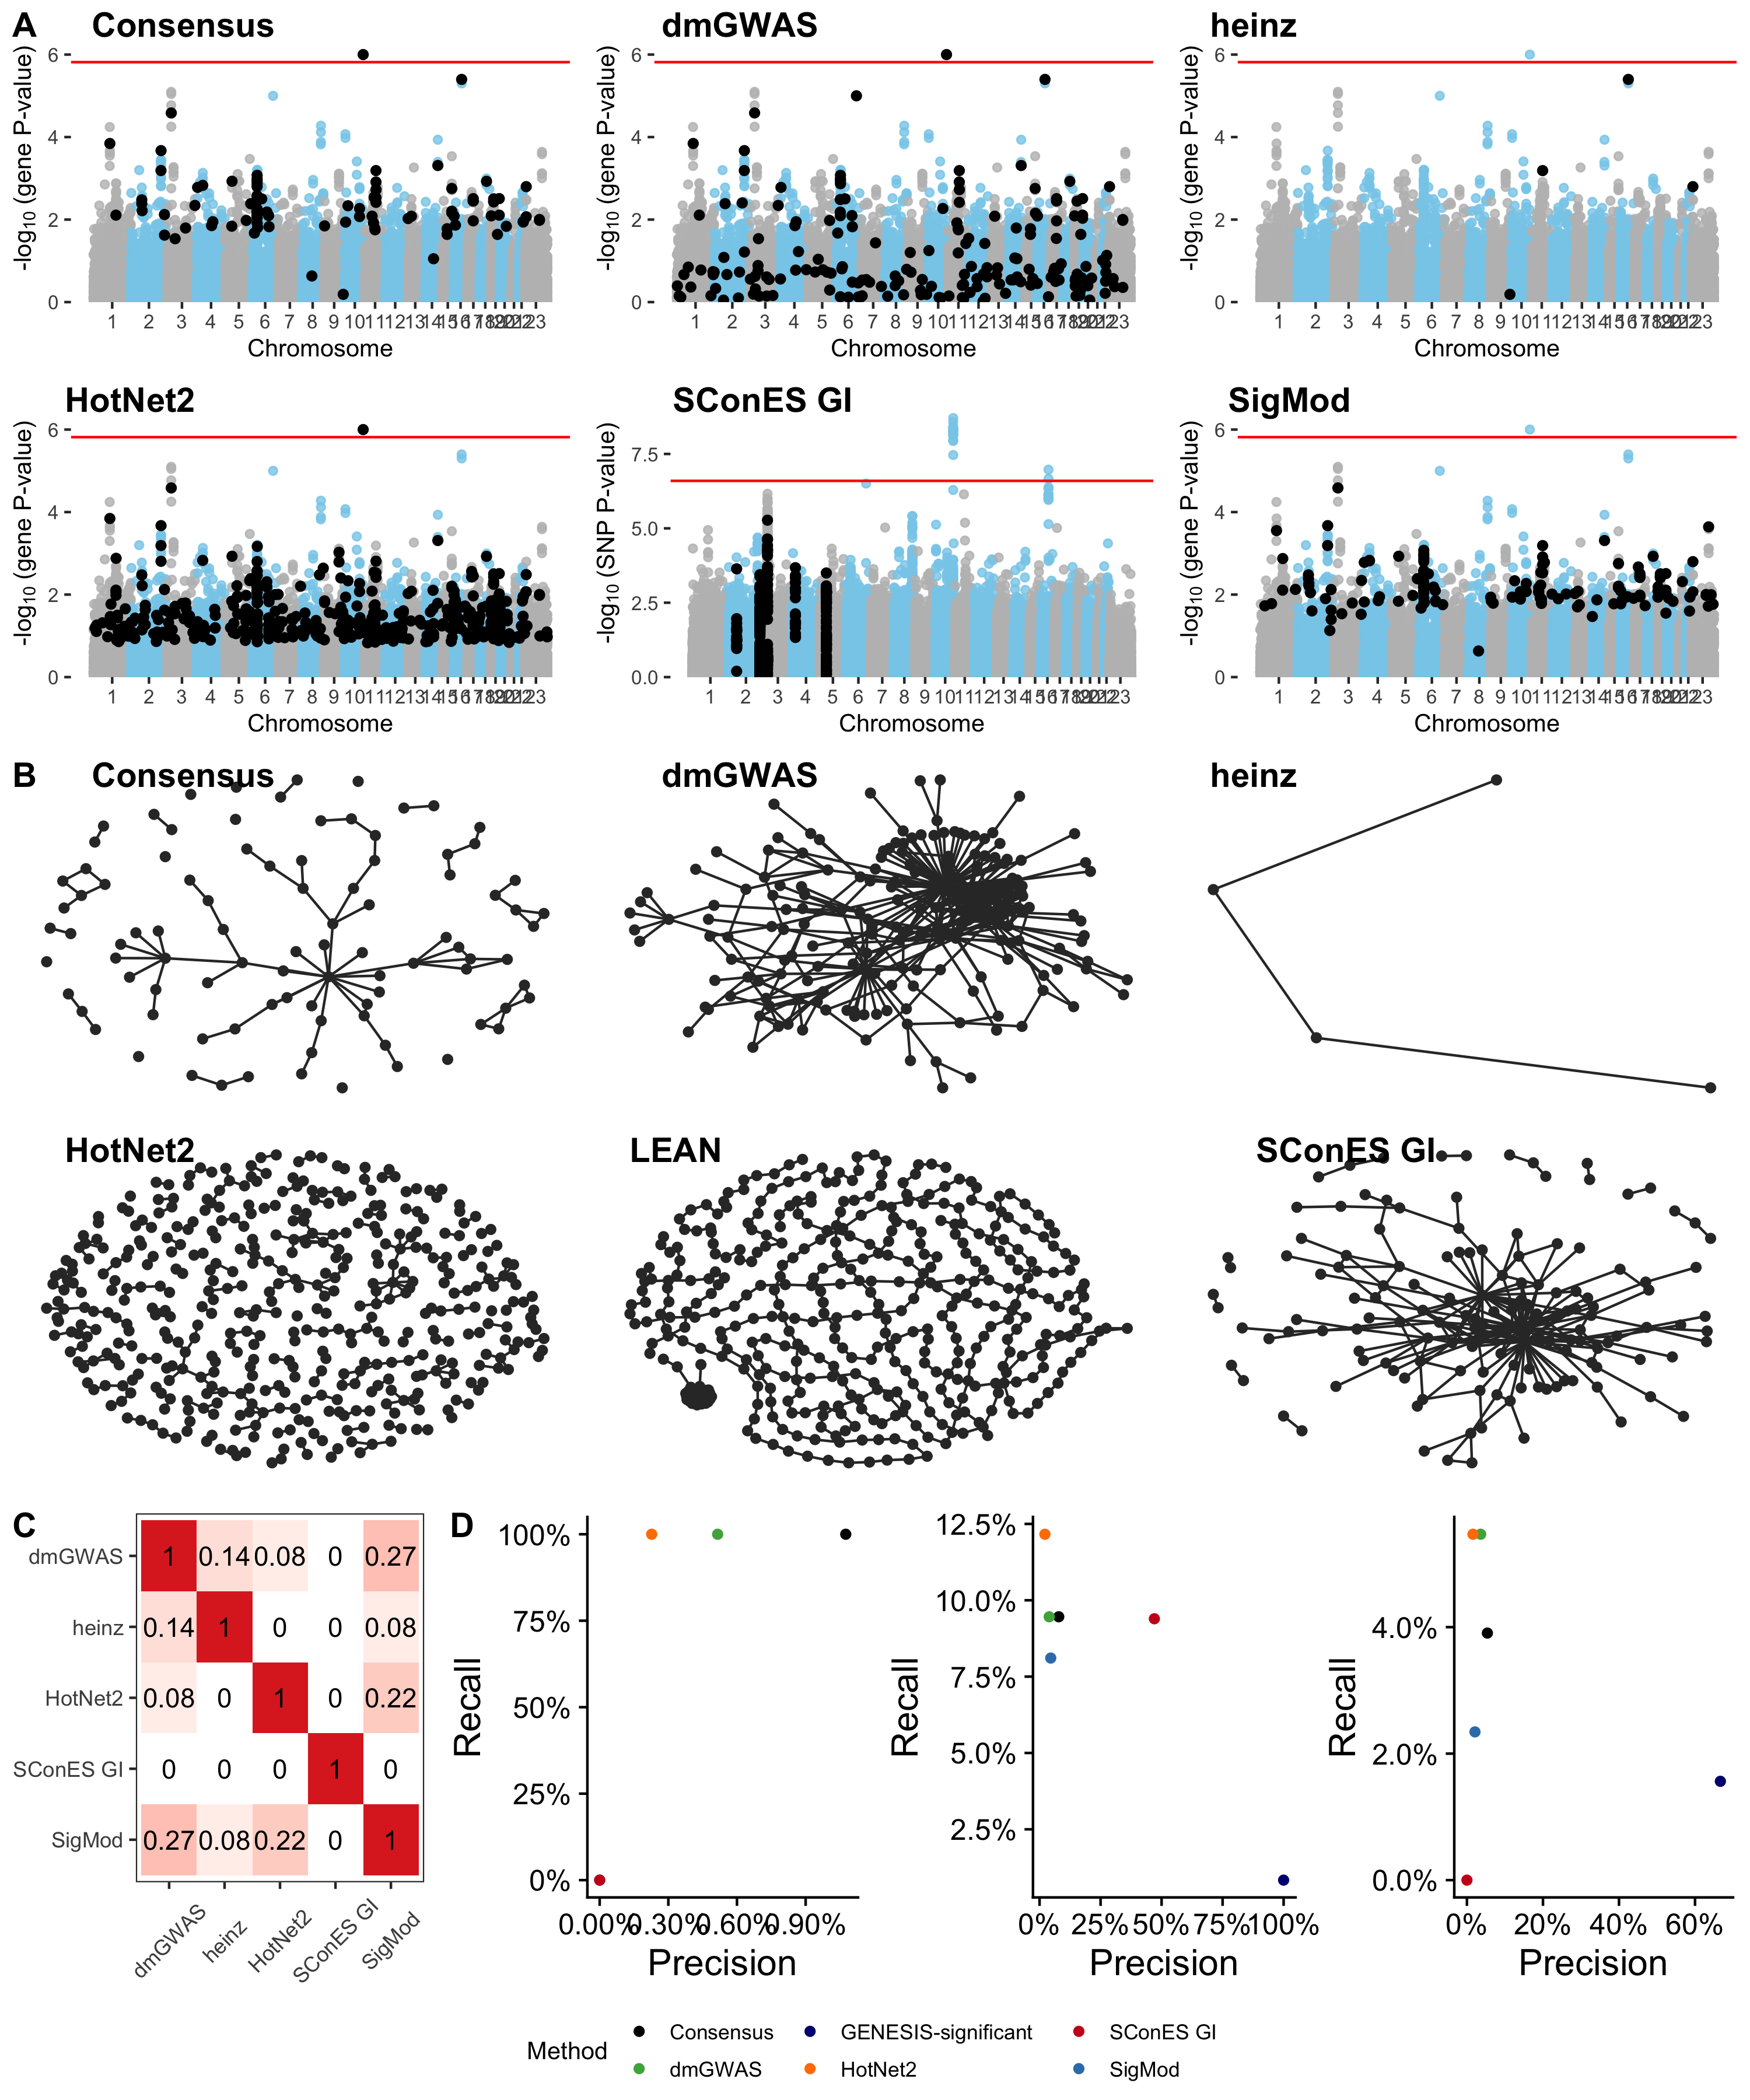
\includegraphics[height=.75\textheight]{./figures/figure_1.png}
  \caption{\label{fig:solution_overview} Overview of the solutions produced by the different network methods (Section~\ref{methods:methods}) on the GENESIS dataset. As LEAN did not produce any significant gene (adjusted P-value < 0.05), it was excluded. Unless indicated otherwise, results refer to genes, except for SConES GI which are at the SNP-level. \textbf{(A)} Manhattan plots of SNPs/genes; in black, the method's solution. The Bonferroni threshold is indicated by a red line (2.54 \texttimes{} 10\textsuperscript{-7} for SNPs, 1.53 \texttimes{} 10\textsuperscript{-6} for genes). \textbf{(B)} \cazcom{\caz{Pearson correlation}{Overlap} between the genes selected by each of the methods\caz{}{, measured by Pearson correlation between indicator vectors}.}{You only explain how to interpret Pearson correlation in Figure 3, although it should maybe come in the Methods when you introduce stability} \textbf{(C)} Precision and recall of the evaluated methods with respect to Bonferroni-significant SNPs/genes in GENESIS (left) and BCAC (middle), and breast cancer susceptibility genes (right, only at the gene-level). For reference, we added a gray line with a slope of 1. \textbf{(D)} Solution networks produced by the different methods.}
\end{figure}

We applied six network methods to the GENESIS dataset (Section~\ref{methods:methods}). As none of the networks examined by LEAN was significant (adjusted P-value < 0.05), we obtained six solutions (Figure~\ref{fig:solution_overview}): one for each of the remaining four gene-based methods, one for SConES GI (which works at the SNP level), and the consensus. \cazcom{TODO Smoothen the transition?}{These solutions differ in many aspects. + go aspect by aspect (size; non-coding regions; topological properties; enriched pathways?} The 4-gene solution selected by heinz includes the breast cancer susceptibility gene \emph{TOX3}, in region 16q12. By dealing with SNP networks, SConES studies the association of non-coding regions, as well as SNPs in any gene, coding or not. In fact, SConES GI retrieves 4 subnetworks in intergenic regions, and 1 overlapping an RNA gene (\emph{RNU6-420P}). SigMod, despite being related to SConES, produces a vastly different, large solution. A pathway enrichment analysis (Section \ref{methods:pathway_enrichment}) links different parts of the network to four processes: protein translation (including mitochondrial), mRNA splicing, protein misfolding, and keratinization (adjusted P-values~<~0.03). Interestingly, dmGWAS solution is also related to protein misfolding (\emph{attenuation phase}, adjusted P-value~=~0.01). But, additionally, it includes submodules of proteins related to mitosis, DNA damage, and regulation of TP53 (adjusted P-values~<~0.49), which match previously known mechanisms of breast cancer susceptibility \cite{nielsen_hereditary_2016}. Lastly, HotNet2 produced 135 subnetworks, 115 of which have less than five genes. The second largest subnetwork (13 nodes) contains the two breast cancer susceptibility genes \emph{CASP8} and \emph{BLM}. As with SigMod, the genes are involved in mitochondrial translation (adjusted P-value~=~1.87 \texttimes{} 10\textsuperscript{-4}), and also in glycogen metabolism and transcription of nuclear receptors (adjusted P-value~<~0.04).

As it can be seen, the solutions are very heterogeneous, making it hard to draw joint conclusions. \caz{In fact, the specific genes by each solution are also different}{The overlap between the genes featured in each solution is quite small} (Figure~\ref{fig:solution_overview}B). Another prominent difference is their sizes: \caz{HotNet2 produced the largest solution (440 genes)}{the largest solution, produced by HotNet2, contains 440 genes,} while SConES GI failed to recover any protein coding gene. Also their topologies differ, as measured by the median centrality and the number of connected components (Figure~\ref{fig:solution_overview}D). 

Yet, some common themes exist \cazcom{(Table~\ref{tab:gene_solutions})}{Why this reference here?}. All obtained solution subnetworks have, \cazcom{on average}{1) you used a median; 2) I'm still wondering if it wouldn't make more sense to report mean or median -log10(p)? The conclusion will still hold}, lower association P-values than the whole PPIN (median P-value $\ll 0.46$), despite containing genes with higher P-values as well (Figure~\ref{fig:solution_overview}A). This exemplifies the trade-off between statistical significance and biological relevance. However, there are nuances between solutions: heinz strongly \caz{}{favors} genes with lower P-values, while dmGWAS is less conservative (median P-values 0.0012 and 0.19, respectively); SConES tended to select whole LD-blocks; and HotNet2 and SigMod were less likely to select low scoring genes. Additionally, the solution subnetworks present other desirable properties. First, five of them were enriched in known breast cancer susceptibility genes (\cazcom{dmGWAS, heinz, HotNet2, and SigMod}{that's 4, not 5??}, Fisher's exact test one-sided P-value < 0.03). Second, the genes in four solution subnetworks display on average a higher betweenness centrality than the rest of the genes, a difference that is significant in four solutions (consensus, dmGWAS, HotNet2, and SigMod, Wilcoxon rank-sum test P-value < 1.4 \texttimes{} 10\textsuperscript{-21}). This agrees with the notion that disease genes are more central than other non-essential genes \cite{pinero_uncovering_2016}, an observation that holds in breast cancer (one-tailed Wilcoxon rank-sum test P-value~=~2.64 \texttimes{} 10\textsuperscript{-5} when comparing the betweenness of known susceptibility genes versus the rest). Interestingly, SConES selected SNPs that are also more central than the average SNP (Supplementary table~\ref{tab:snp_solutions}), suggesting that causal SNPs are also more central than non associated SNPs. However, very central nodes are also more likely to be connecting a given random pair of nodes, making them more likely to be selected by \caz{the examined}{any network} methods. \cazcom{Hence, further work is needed characterize the impact of centrality on these methods' \caz{results}{outputs}.}{Maybe more of a Discussion than a Results sentence?}

\subsection{A case study: the consensus network}
\label{results:consensus}
\begin{figure}[htbp]
  \centering
  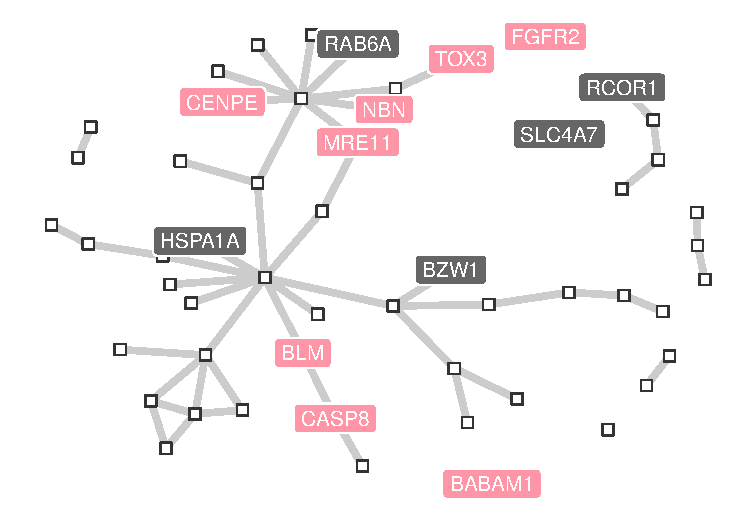
\includegraphics[width=.5\linewidth]{./figures/figure_3.pdf}
  \caption{\label{fig:consensus}
    Consensus subnetwork on GENESIS (Section~\ref{methods:methods}). Each node is represented by a pie chart, which shows the methods that selected it. We labeled (and enlarged) the genes having a VEGAS2v2 P-value < 0.001, the two most central genes (\emph{COPS5} and \emph{OFD1}) and those that are known breast cancer susceptibility genes. The latter ones are also colored in pink.}
\end{figure}

\caz{The shared properties despite their heterogeneity suggested that each method was capturing}{Despite the heterogeneity of the solutions, their shared properties suggest that each method captures} different aspects of cancer susceptibility. Indeed, only 20 genes \caz{were}{are} common to more than two solutions (Supplementary Figure~\ref{sfig:consensus_stats}A), but encouragingly, the more methods select\caz{ed}{} a gene, the higher its association \caz{was}{to the phenotype} (Supplementary Figure~\ref{sfig:consensus_stats}B). To leverage on their strengths and compensate their respective weaknesses, we built a consensus subnetwork that captures the mechanisms most shared among the solution subnetworks (Section~\ref{methods:methods}). This subnetwork (Figure~\ref{fig:consensus}) contains 93 genes and shares the aforementioned properties of the individual solutions: enrichment in breast cancer susceptibility genes and higher betweenness centrality than the rest of the genes. 

A pathway enrichment analysis of the genes in the consensus network also shows similar pathways as the individual solutions. \cazcom{After tackling the overlap between the significant pathways}{I'm not sure what you mean here?}, we found two involved mechanisms: \emph{mitochondrial translation} and \emph{attenuation phase}. The former is supported by genes like \emph{MRPS30} (VEGAS P-value~=~0.001), which encode a mitochondrial ribosomal protein and was also linked to breast cancer susceptibility \cite{quigley_5p12_2014}. Interestingly, increased mitochondrial translation has been found in cancer cells \cite{Yu2016Repositioning}, and its inhibition proposed as a therapeutic target. With regards to attenuation phase of heat shock response, it involves three Hsp70 chaperones: \cazcom{HSPA1A, HSPA1B, and HSPA1L}{Italics for gene/protein names? Or is it only for gene names? But HSPA1A is in italics below.}. The genes encoding these proteins are all near each other at \cazcom{6p21}{Isn't that the HLA complex? I'm always a bit wary of this region because of the strong LD, disantangling signals is hard...}. In fact, out of the 22 SNPs that map to any of these three genes, 9 map to all of them, and 4 to two, making hard to disentangle their association. \emph{HSPA1A} was the most strongly associated one (VEGAS P-value~=~8.37 \texttimes{} 10\textsuperscript{-4}).  

Topologically the consensus consists of a connected component composed of 49 genes, and multiple smaller subnetworks. Among the latter, 14 of the 93 genes are in subnetworks containing a single gene or two connected nodes, implying that they do not have a consistently altered neighborhood, but are strongly associated themselves and hence picked by two methods. The opposite would be the case of genes with highly centrality in the PPIN, which is weakly anti-correlated with the P-value of association to the disease (Pearson correlation coefficient~=~-0.26, Supplementary Figure~\ref{sfig:consensus_stats}D). This suggests that they were selected because they were on the shortest path between two highly associated genes. In view of this, we hypothesize that highly central genes might contribute to the heritability through consistent alterations of their neighborhood, consistent with the omnigenic model of disease \cite{boyle_expanded_2017}. For instance, the most central node in the consensus network is \emph{COPS5}, a gene related to multiple hallmarks of cancer and which is overexpressed in multiple tumors, including breast and ovarian cancer \cite{liu_jab1_cops5_2018}. Despite its lack of association in GENESIS or BCAC (VEGAS2v2 P-value of 0.22 and 0.14 respectively), its neighbors in the consensus subnetwork have consistently low P-values (median VEGAS2v2 P-value~=~0.006).

\subsection{Methods are comparably unstable, and produce similar predictors}
\cazcom{}{1) ``Network methods'' rather than ``Methods'' in title? 2) I'm not sure we want to emphasize predictor similarity when they're all so terrible 3) Shouldn't this section appear before the previous one? First talk about the individual solutions, then present the consensus?.}

\begin{figure}[htbp]
\centering
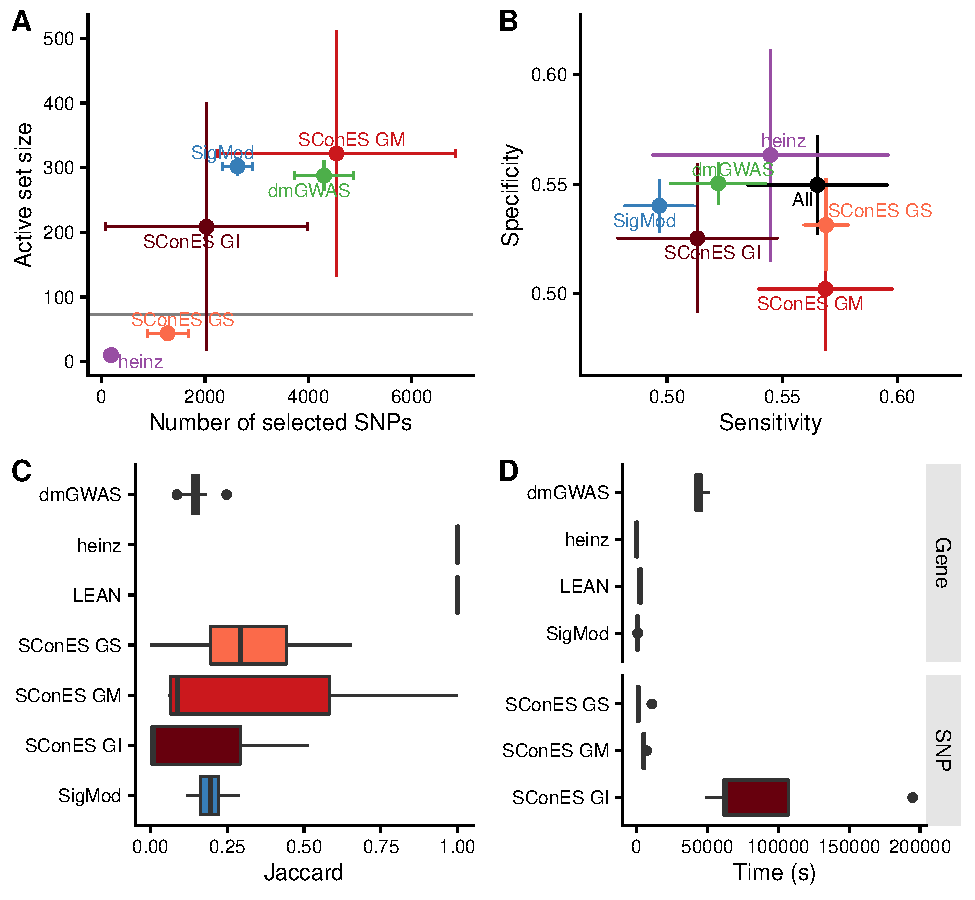
\includegraphics[width=.72\linewidth]{./figures/figure_4.pdf}
\caption{\label{fig:benchmark}
Comparison of network-based GWAS methods on GENESIS. Each method was run 5 times \caz{of}{on} a random subset of the samples, and tested on the remaining samples (Section \ref{methods:comparison}). As LEAN did not select any gene, it was excluded from all panels except \textbf{D}. \textbf{(A)} Number of SNPs selected by each method \cazcom{and number of SNPs in the active set \caz{used}{found} by the \caz{Lasso}{L1-penalized logistic regression} classifier}{Not necessary if L1-penalized logreg is introduced in the Methods}. Points are the average over the 5 runs; lines represent the standard error of the mean. A grey diagonal line with slope 1 is added for comparison. For reference, the active set of Lasso using all the SNPs included, on average, 154\,117.4 SNPs. \textbf{(B)} Sensitivity and specificity on test set of the L1-penalized logistic regression trained on the features selected by each of the methods. In addition, the performance of the classifier trained on all SNPs is displayed. Points are the average over the 5 runs; lines represent the standard error of the mean. \textbf{(C)} Pairwise Pearson correlations of the solutions used by different methods. A Pearson correlation of 1 means the two solutions are the same. A Pearson correlation of 0 means that there is no SNP in common between the two solutions. \textbf{(D)} Runtime of the evaluated methods, by type of network used (gene or SNP). For gene network-based methods, inverted triangles represent the runtime of the algorithm itself, and circles the total time, which includes the algorithm themselves and the additional 119\,980 seconds (1 day and 9.33 hours) \caz{which took VEGAS2v22}{that VEGAS2v2 took} on average to compute the gene scores from SNP summary statistics.}
\end{figure}

We compared the six \caz{}{network} methods in a 5-fold subsampling setting (Section \ref{methods:comparison}). Specifically, we measured five properties (Figure~\ref{fig:benchmark}): size of the solution subnetwork; sensitivity and specificity of an L1-penalized logistic regression classifier on the selected SNPs; stability; and computational runtime. Both solution size and the subset of it selected by the classifier (\emph{active set}) varies greatly between the different methods (Figure~\ref{fig:benchmark}A). Heinz produced the smallest solutions, with an average of 182 selected SNPs. The largest solutions come from SConES GI (6\,256.6 SNPs), and dmGWAS (4\,255.0 SNPs). Interestingly, \cazcom{heinz has the highest proportion of the selected SNPs that go into the active set (99.9\%)}{Isn't that because it's only selecting 4 genes?}, although \caz{it}{this proportion} is high for all the methods (> 86\%). To determine whether the selected SNPs could be used for patient classification, we computed the performance of the classifier on the \emph{test dataset} (Figure~\ref{fig:benchmark}B). The different classifiers displayed similarly poor sensitivities and specificities, all in the 0.52 -- 0.56 range. Interestingly, the classifier trained on all the SNPs had a similar performance, despite being the only method \caz{whose stated goal is to minimize}{aiming only at minimizing} prediction error. \cazcom{}{Do we want to comment this suggest that in any case there isn't that much signal in the data set, or are we shooting ourselves in the foot doing that?}

Another desirable quality of an algorithm is the stability of the solution with regards to small changes in the input (Section~\ref{methods:algorithm_comparison}). Both heinz and LEAN displayed a high stability in our benchmark, consistently selecting the same genes and no genes over the 5 subsamples, respectively (Figure~\ref{fig:benchmark}C). Conversely, the other methods displayed similarly low stabilities. 

In terms of computational runtime, the fastest method was heinz (Figure~\ref{fig:benchmark}D), which \caz{leverages on its ability to find efficiently the solution}{finds the solution efficiently} in a few seconds. HotNet2 was the slowest (3 days and 14 hours on average). Including the time required to compute the gene scores, however, slows down considerably gene-based methods; on this benchmark, that step took on average 1 day and 9.33 hours. Considering that, it took 5 days on average for HotNet2 to produce a result.

\subsection{The consensus overcomes the problems of the individual solutions}
\label{results:drawbacks}

\begin{figure}[htbp]
\centering
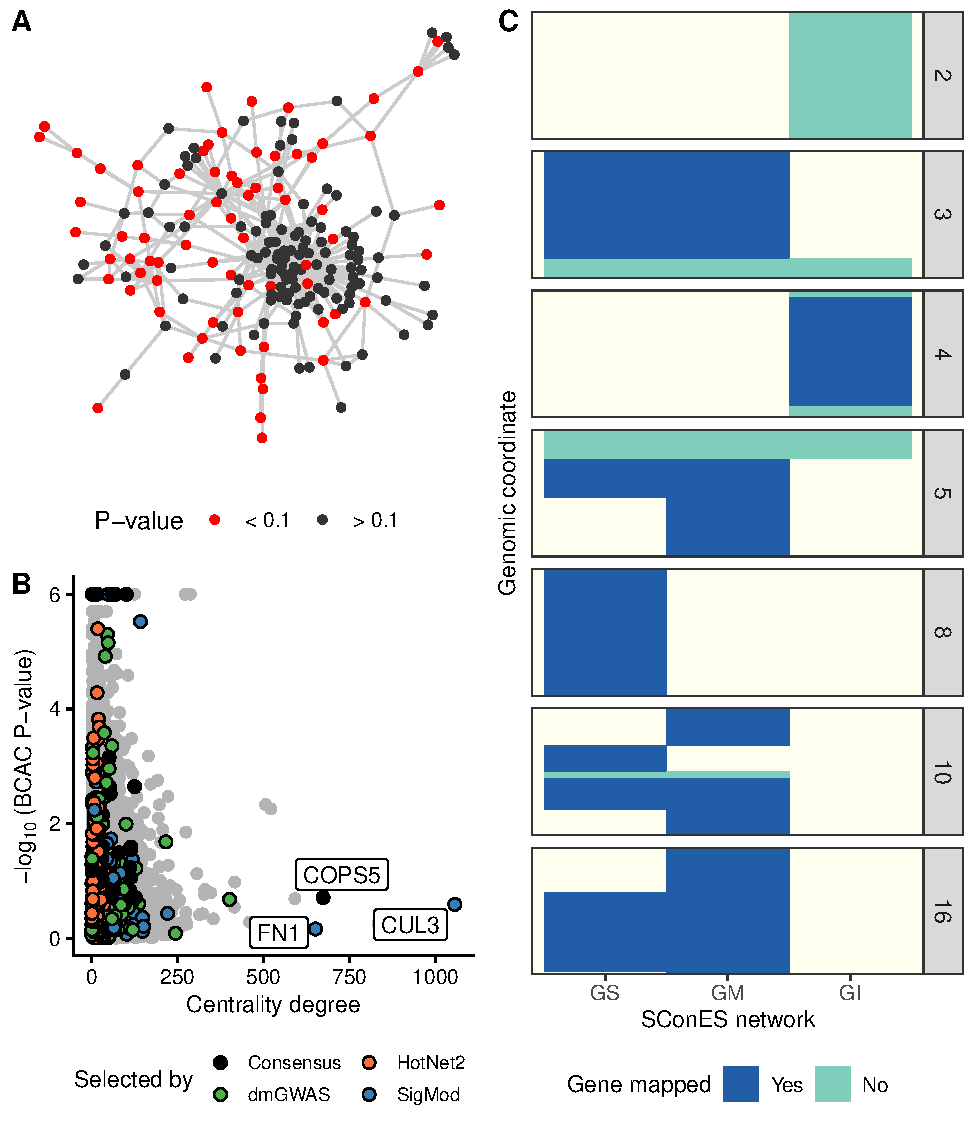
\includegraphics[width=.8\linewidth]{./figures/figure_2.pdf}
\caption{\label{fig:issues}
Drawbacks \caz{confronted}{encountered?} when using network guided methods. \textbf{(A)} dmGWAS solution subnetwork. Genes with a P-value < 0.1 are highlighted in red. \textbf{(B)} Centrality degree and -log\textsubscript{10} of the VEGAS2v2 P-value for the nodes in SigMod solution subnetwork. \textbf{(C)} Genomic regions where either SConES GS, GM or GI select SNPs.}
\end{figure}

\cazcom{In practice, and despite their similarities and their involvement in cancer mechanisms, the solutions are remarkably different. That is due to the particularities of the methods which directly or indirectly provide information about the dataset. For instance, the fact that LEAN did not provide any biomarkers implies that there is no gene such that both itself and its environment are on average strongly associated with the disease.}{Slightly redundant with the ``A case study: the consensus network'' section, and also maybe move the sentence about LEAN to that section?}

\cazcom{}{Also the first few paragraphs of this section are somewhat redundant with the ``A case study: the consensus network'' section?}

In this dataset, heinz's solution is very conservative, providing a small solution with the lowest median P-value for the subnetwork (Table~\ref{tab:gene_solutions}). Due to this parsimonious and highly associated solution, it was the best method to stably select a set of biomarkers (Figure~\ref{fig:benchmark}C). Its conservativeness stems from its preprocessing step, which models the gene P-values as a mixture model of a beta and a uniform distribution, controlled by an FDR parameter. Due to the limited signal at the gene level in this dataset (Supplementary Figure~\ref{sfig:snp_gene_manhattan}B), only 36 of them are retain a positive score after that transformation. This small solution does not provide much insight of the biology of cancer. Importantly, it ignores genes that are associated to cancer in this dataset like \emph{FGFR2}. 

On the other end of the spectrum, we have large solutions provided by dmGWAS, HotNet2, and SigMod. dmGWAS' subnetwork is the least associated subnetwork on average. This is due to the greedy framework it uses, which has a bias for larger solutions \cite{nikolayeva_network_2018}. This framework considers all nodes at distance 2 of the examined, and accepts weakly associated genes if they are linked to another, strongly associated one. This is exacerbated when the results of successive greedy searches are aggregated, leading to a large, tightly connected cluster of unassociated genes (Figure~\ref{fig:issues}A). SigMod displays the same tendency, as the most central genes are the least associated to the disease (Figure~\ref{fig:issues}B). This relatively low signal-to-noise ratio combined with the large solution requires additional analyses to draw conclusions, such as enrichment analyses. In the same line, HotNet2's subnetwork is even harder to interpret, being composed of 440 genes divided into 135 subnetworks. Lastly, SigMod misses some of the most strongly associated, breast cancer susceptibility genes in the dataset, like \emph{FGFR2} and \emph{TOX3}.

By virtue of using a SNP subnetwork, SConES analyzes each SNP in their context. It therefore selects SNPs in genes none of whose interactors are associated to the disease, as well as SNPs in non-coding regions or in non-interacting genes. In fact, due to linkage disequilibrium, such genes are favored by SConES, as selecting SNPs in an LD block which overlaps with a gene favors selecting the rest of the gene. This might explain why SConES produces similar results on the GS and GM networks, heavily affected by linkage disequilibrium (Supplementary Figure~\ref{sfig:pearson_methods}). On the other hand, SConES penalizes selecting SNPs and not their neighbors. This makes it conservative regarding SNPs with many interactions, for instance those mapped to hubs in the PPIN. For this reason, SConES GI did not select any protein coding gene, despite selecting similar regions as SConES GS (Figure~\ref{fig:issues}C). In fact SConES GS and SConES GM select regions related to breast cancer, like 16q12 (\emph{TOX3}, Section~\ref{results:conventional}), 3p24 (\emph{SLC4A7}/\emph{NEK10} \cite{ahmed_newly_2009}), 5p12 (\emph{FGF10}, \emph{MRPS30} \cite{quigley_5p12_2014}), and 10q26 (\emph{FGFR2}, Section~\ref{results:conventional}). On top of that only SConES GS selects region 8q24 (\emph{POU5F1B} \cite{breyer_expressed_2014}). We hypothesize that the lack of results on the PPIN network of SConES GI and LEAN are due to the same cause: the absence of joint association of a module. Although in the case of SConES other hyperparameters could lead to a more informative solution (e.g. lower \(\lambda\), Section~\ref{methods:methods}), it is unclear what is the best strategy to find them. In addition, due to the iCOGS SNP array design, the genome of GENESIS participants has not been unbiasedly surveyed: some regions are fine-mapped --- which might distort gene structure in GM and GI networks --- while others are under studied --- hurting the accuracy with which the GS network captures the genome structure.

\subsection{Network methods boost biomarker discovery}

We compared the results of different network methods to the European cohort of the Breast Cancer Association Consortium (BCAC) \cite{Michailidou2017}, the largest GWAS to date in breast cancer (Section~\ref{methods:bcac}). This comparison is pertinent as, despite not targeting the same population(s), we expect a shared genetic architecture at the gene level % \cite{required}
TODO CAN'T FIND A CITATION FOR THIS, at which most examined network metods operate. This shared genetic architecture, together with BCAC's scale (90 times more samples than GENESIS) provides a reasonable counterfactual of what we would expect if GENESIS had a larger sample size. We computed a gene association score on BCAC, in an equivalent way to the one described in Section~\ref{methods:node_score}. The solutions provided by the different network approaches overlap significantly (Fisher's exact test P-value \textless~0.019). The gene-based methods achieve comparable precision (2\%-25\%) and recall (1.3-12.1\%) (Figure~\ref{fig:solution_overview}C). However, while SConES GI at the SNP-level achieves a similar recall (8.6\%), it shows a much higher precision (47.3\%).

\section{Discussion}

In this article we evaluate the viability of a systems biology take on genetic studies by examining a GWAS dataset on familial breast cancer. Such an approach addresses two of the largest issues with GWAS: interpretability and an overly conservative statistical framework that hinders discovery. This is achieved by considering the biological context of each of the genes and SNPs. Based on divergent considerations of what the desired set of biomarkers is, several methods for network-guided biomarker discovery have been proposed. We reviewed six of them. Most of them produced a relevant subset of biomarkers, although the solutions were notably different. In one end of the spectrum, SConES and heinz preferred small, highly associated solutions, providing a conveniently short list of biomarkers, at the expense of not shedding much light on the etiology of the disease. On the other end, SigMod and dmGWAS gravitate towards larger, less associated solutions which provide a wide overview of the biological context. While this deepens our understanding of the disease and provide biological hypotheses, they require further analyses, which risk oversimplifying their richness. HotNet2 balances both approaches at the expense of producing the largest solution: a constellation of many, highly associated, small subnetworks. Despite these differences, all the solutions produced comparably poor discrimination capabilities on a linear classifier trained on them, and were remarkably unstable, and hence likely to produce change in face of slightly different inputs.

To overcome the problems posed by the individual methods while exploiting their strengths, we propose combining them into a consensus subnetwork. We use a straightforward aggregation to generate it, including any node that was recovered by at least two methods. The resulting network is a synthesis of the altered mechanism: it is smaller than the largest solutions (HotNet2, SigMod and dmGWAS), which makes it more manageable, and includes the majority of the strongly associated smaller solutions (SConES and heinz). The consensus subnetwork captures mechanisms and genes known to be related to cancer, recovering known breast cancer susceptibility genes as well as genome regions associated to breast cancer susceptibility. However, thanks to its smaller size and its network structure, it provides compelling hypotheses of non-canonical mechanisms involved in carcinogenesis, like mitochondrial translation and chaperone activity.

The strength of network-based analyses comes from leveraging prior knowledge to boost discovery. In consequence, they show their shortcomings in front of understudied genes, especially those not in the network. Out of the 32\,767 genes that we can map the genotyped SNPs to, 60.7\% (19\,887) are not in the protein-protein interaction network. The majority of those (14\,660) are non-coding genes, mainly lncRNA, miRNA, and snRNA (Supplementary Figure~\ref{sfig:biotypes_excluded}). Yet, RNA genes like \emph{CASC16} are associated to breast cancer (Section~\ref{results:conventional}), reminding us of the importance of using networks beyond coding genes. Even protein-coding genes linked to breast cancer susceptibility \cite{ahmed_newly_2009}, like \emph{NEK10} (P-value 1.6 \texttimes{} 10\textsuperscript{-5}, located near \emph{SLC4A7}) or \emph{POU5F1B}, were absent from the network. However, on average protein-coding genes absent from the PPIN are less associated with this phenotype (Wilcoxon rank-sum P-value~=~2.79 \texttimes{} 10\textsuperscript{-8}, median P-values of 0.43 and 0.47). As we are using interactions from high-throughput experiments, such difference cannot be due to well-known genes having more known interactions. As disease genes tend to be more central \cite{pinero_uncovering_2016}, we hypothesize that it is due to interactions between central genes being more likely. It is worth noting that network approaches that do not use PPIs, like SConES GS and GM, did recover SNPs in \emph{NEK10} and \emph{CASC16}. This shows the potential of SNP networks, in which SNPs are linked when there is evidence of co-function, to perform network-guided GWAS even in the absence of gene-level interactions. Lastly, all the methods rely heavily on how SNPs are mapped to genes. In Section~\ref{results:consensus} we highlight ambiguities that appear when genes overlap or are in linkage disequilibrium.

As not all databases compile the same interactions, the choice of the PPIN determines the final output. In this work we used exclusively interactions from HINT from high-throughput experiments. This responds to concerns of some authors about adding interactions identified in targeted studies and prone to a ``rich getting richer'' phenomenon: popular genes have a higher proportion of their interactions described \cite{cai_broker_2010,das_hint:_2012}. Their presense might bias the results of the presented methods, as they change the topology of the network by adding nodes closer to other nodes than average. On the other hand, \citet{huang_systematic_2018} found that the best predictor of the performance of a network for disease gene discovery is the size of the network, which supports using the largest amount of interactions. When we compared the impact of using a larger network containing interactions from both high-throughput experiment and the literature (Section~\ref{methods:networks}), we found that for most of the methods it did not greatly change the size or the stability of the solution, the classification accuracy, or the runtime (Supplementary Figure~\ref{sfig:lc_ht_comparison}). This supports using only interactions from high-throughput experiments, which produces apparently similar solutions and avoids falling into ``circular reasonings'', where the best known genes are artificially pushed into the selected solutions. 

A crucial step for the gene based methods is the computation of the gene score. In this work we used VEGAS2v2 \cite{mishra_vegas2:_2015} due to the flexibility it offers to use user-specified gene annotations. However, it presents known problems (selection of an appropriate percentage of top SNPs, long runtimes and P-value precision limited to the number of permutations \cite{nakka_gene_2016}), and other algorithms might have more statistical power. Another important decision is how to handle LD in a GWAS. VEGAS2v2 accounts for LD patterns, and hence an LD pruning step would not impact gene-based network methods, although it would speed up VEGAS2v2's computation time. With regards to SConES, less SNPs would lead to simpler SNP networks and, possibly, shorter runtimes. However, as mentioned in Section~\ref{results:drawbacks}, LD patterns seem paramount to SConES' solutions, and an LD pruning step could potentially alter them. 

In order to produce the consensus network, we had to face the different interfaces, preprocessing steps, and unexpected behaviors of the various methods. To facilitate that other authors apply them to new datasets and aggregate their solutions, we built six nextflow pipelines \cite{di_tommaso_nextflow_2017} with a consistent interface and, whenever possible, parallelized computation. They are available on GitHub: \url{https://github.com/hclimente/gwas-tools}. Importantly, those methods that had a permissive license were compiled into a Docker image for easier use, which is available on Docker Hub \href{https://hub.docker.com/r/hclimente/gwas-tools}{hclimente/gwas-tools}.

\section*{Author contributions}

H.C-G. conducted all the final analyses and the writing of the manuscript. C.L. conducted analyses using LEAN, Sigmod, and dmGWAS, and provided help and feedback. F.L. and N.A. provided feedback on the analyses and the manuscript. C-A.A. supervised the project.

\section*{Funding and acknowledgments}

This project was supported by funding from Agence Nationale de la Recherche (ANR-18-CE45-0021-01) and from the European Union’s Horizon 2020 research and innovation program (Marie Skłodowska-Curie [666003]). Financial support for GENESIS resource and genotyping was provided by the Ligue Nationale contre le Cancer (grants PRE05/DSL, PRE07/DSL, PRE11/NA), the French National Institute of Cancer (INCa grant b2008-029/LL-LC) and the comprehensive cancer center SiRIC (Site de Recherche Intégrée sur le Cancer: INCa-DGOS-4654).

We wish to thank the genetic epidemiology platform (the PIGE, Plateforme d'Investigation en Génétique et Epidemiologie: O. Kulkarni, S. Eon-Marchais, M. Marcou, D. Le Gal, L. Toulemonde, J. Beauvallet, N. Mebirouk, E. Cavaciuti), the biological resource centre (S. Mazoyer, F. Damiola, L. Barjhoux, C. Verny-Pierre, V. Sornin) and all the GENESIS collaborating cancer clinics clinics (Clinique Sainte Catherine, Avignon: H. Dreyfus; Hôpital Saint Jacques, Besançon: M-A. Collonge-Rame; Institut Bergonié, Bordeaux: M.Longy, A. Floquet, E. Barouk-Simonet; CHU, Brest: S. Audebert; Centre François Baclesse, Caen: P. Berthet; Hôpital Dieu, Chambéry: S. Fert-Ferrer; Centre Jean Perrin, Clermont-Ferrand: Y-J. Bignon; Hôpital Pasteur, Colmar: J-M. Limacher; Hôpital d’Enfants CHU – Centre Georges François Leclerc, Dijon: L. Faivre-Olivier; CHU, Fort de France: O. Bera; CHU Albert Michallon, Grenoble: D. Leroux; Hôpital Flaubert, Le Havre: V. Layet; Centre Oscar Lambret, Lille: P. Vennin, C. Adenis; Hôpital Jeanne de Flandre, Lille: S. Lejeune-Dumoulin, S. Manouvier-Hanu; CHRU Dupuytren, Limoges: L. Venat-Bouvet; Centre Léon Bérard, Lyon: C. Lasset, V. Bonadona; Hôpital Edouard Herriot, Lyon: S. Giraud; Institut Paoli-Calmettes, Marseille: F. Eisinger, L. Huiart; Centre Val d’Aurelle – Paul Lamarque, Montpellier: I. Coupier; CHU Arnaud de Villeneuve, Montpellier: I. Coupier, P. Pujol; Centre René Gauducheau, Nantes: C. Delnatte; Centre Catherine de Sienne, Nantes: A. Lortholary; Centre Antoine Lacassagne, Nice: M. Frénay, V. Mari; Hôpital Caremeau, Nîmes: J. Chiesa; Réseau Oncogénétique Poitou Charente, Niort: P. Gesta; Institut Curie, Paris: D. Stoppa-Lyonnet, M. Gauthier-Villars, B. Buecher, A. de Pauw, C. Abadie, M. Belotti; Hôpital Saint-Louis, Paris: O. Cohen-Haguenauer; Centre Viggo-Petersen, Paris: F. Cornélis; Hôpital Tenon, Paris: A. Fajac; GH Pitié Salpétrière et Hôpital Beaujon, Paris: C. Colas, F. Soubrier, P. Hammel, A. Fajac; Institut Jean Godinot, Reims: C. Penet, T. D. Nguyen; Polyclinique Courlancy, Reims: L. Demange, C. Penet; Centre Eugène Marquis, Rennes: C. Dugast; Centre Henri Becquerel, Rouen: A. Chevrier, T. Frebourg, J. Tinat, I. Tennevet, A. Rossi; Hôpital René Huguenin/Institut Curie, Saint Cloud: C. Noguès, L. Demange, E. Mouret-Fourme; CHU, Saint-Etienne: F. Prieur; Centre Paul Strauss, Strasbourg: J-P. Fricker, H. Schuster; Hôpital Civil, Strasbourg: O. Caron, C. Maugard; Institut Claudius Regaud, Toulouse: L. Gladieff, V. Feillel; Hôpital Bretonneau, Tours: I. Mortemousque; Centre Alexis Vautrin, Vandoeuvre-les-Nancy: E. Luporsi; Hôpital de Bravois, Vandoeuvre-les-Nancy: P. Jonveaux; Gustave Roussy, Villejuif: A. Chompret, O. Caron). 


\cazcom{}{TODO Clean out references a bit (remove URLs, shorten long authors lists with et al., etc.)}

\bibliographystyle{abbrvnat}
\bibliography{bibliography}

\clearpage
\setcounter{figure}{0}
\setcounter{section}{0}
\setcounter{table}{0}

\section{Supplementary materials}

\begin{table}[htbp]
\begin{threeparttable}
\caption{\label{tab:snp_solutions}
Summary statistics on the results of SConES on the three SNP-SNP interaction networks. The first row within each block contains the summary statistics on the whole network.}
\centering
\begin{tabular}{lrrllr}
Network & SNPs & Edges & Subnetworks & \mean{Betweenness} & \median{P}\textsubscript{SNP}\\
\hline
GS & 197\,083 & 197\,060 & - & 2.03 \texttimes{} 10\textsuperscript{7} & 0.49\\
SConES GS & 1\,590 & 1\,585 & 5 & 2.52 \texttimes{} 10\textsuperscript{7} & 0.023\\
\hline
GM & 197\,083 & 6\,442\,446 & - & 3.99 \texttimes{} 10\textsuperscript{6} & 0.49\\
SConES GM & 1\,692 & 177\,611 & 5 & 4.40 \texttimes{} 10\textsuperscript{6} & 0.055\\
\hline
GI & 197\,083 & 28\,733\,720 & - & 1.46 \texttimes{} 10\textsuperscript{6} & 0.49\\
SConES GI & 408 & 539 & 5 & 9.33 \texttimes{} 10\textsuperscript{6} & 0.076\\
\end{tabular}
\begin{tablenotes}
  \footnotesize{
    \item \mean{Betweenness}: mean betweenness of the selected SNPs in the corresponding full network.\median{P}\textsubscript{SNP}: median P-value of the selected SNPs.
  }
\end{tablenotes}
\end{threeparttable}
\end{table}

\begin{table}[htbp]
\begin{threeparttable}
  \caption{\label{tab:scones_gene_solutions}
Summary statistics on the results of multiple network methods on the gene-gene interaction network. The first row contains the summary statistics on the whole network.}
\centering
\begin{tabular}{lrrrlr}
Network & Genes & Edges & \mean{Betweenness} & \median{P}\textsubscript{gene} & $\rho_{consensus}$\\
\hline
SConES GS & 5 & 0 & 9\,805 & 2.7 \texttimes{} 10\textsuperscript{-5} & 0.19\\
SConES GM & 28 & 2 & 4\,267 & 0.067 & 0.12\\
\end{tabular}
\begin{tablenotes}
  \footnotesize{
    \item \mean{Betweenness}: mean betweenness of the selected genes in the full network. \median{P}\textsubscript{gene}: median P-value of the selected genes; $\rho_{consensus}$: Pearson correlation with the consensus network.
  }
\end{tablenotes}
\end{threeparttable}
\end{table}

\begin{figure}[htbp]
\centering
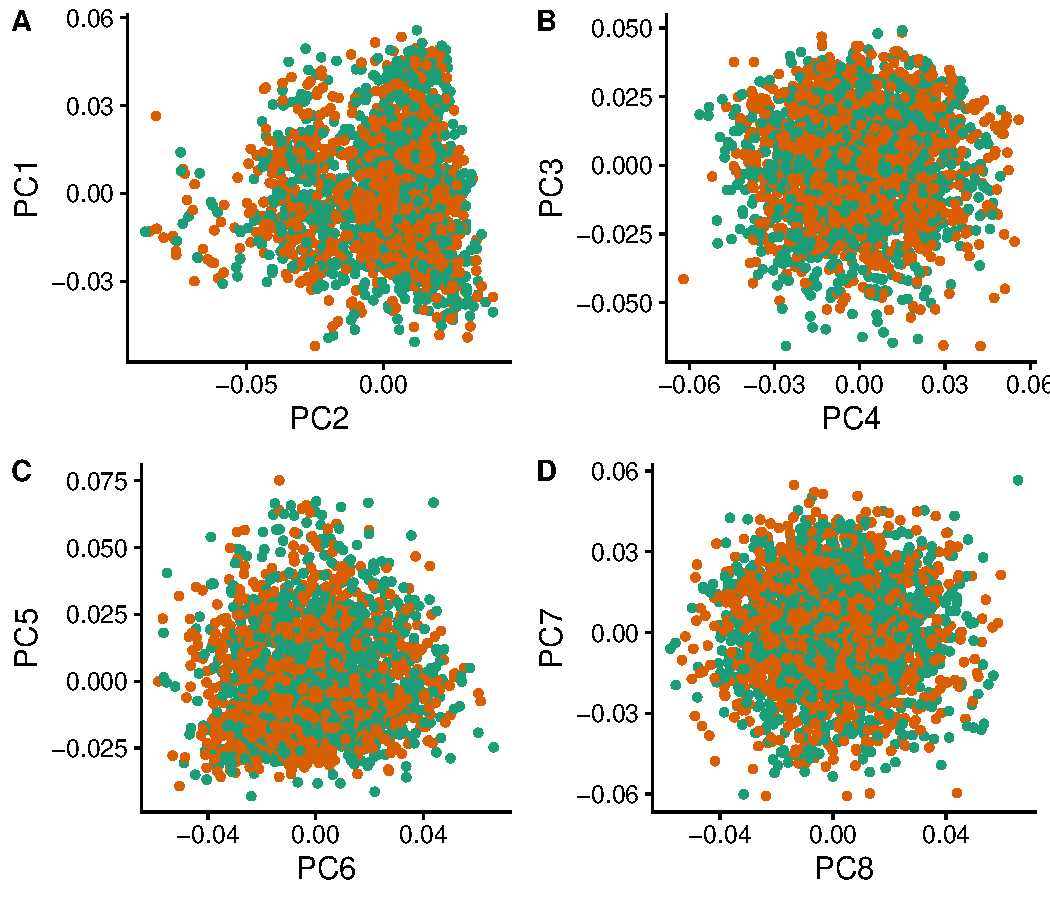
\includegraphics[width=.9\linewidth]{./figures/sfigure_1.pdf}
\caption{\label{sfig:pcs} GENESIS shows no differential population structure between cases and controls. \textbf{(A,B,C,D)} Eight main principal components computed on the genotypes of GENESIS. Cases are colored in green, controls in orange.}
\end{figure}

\begin{figure}[htbp]
  \centering
  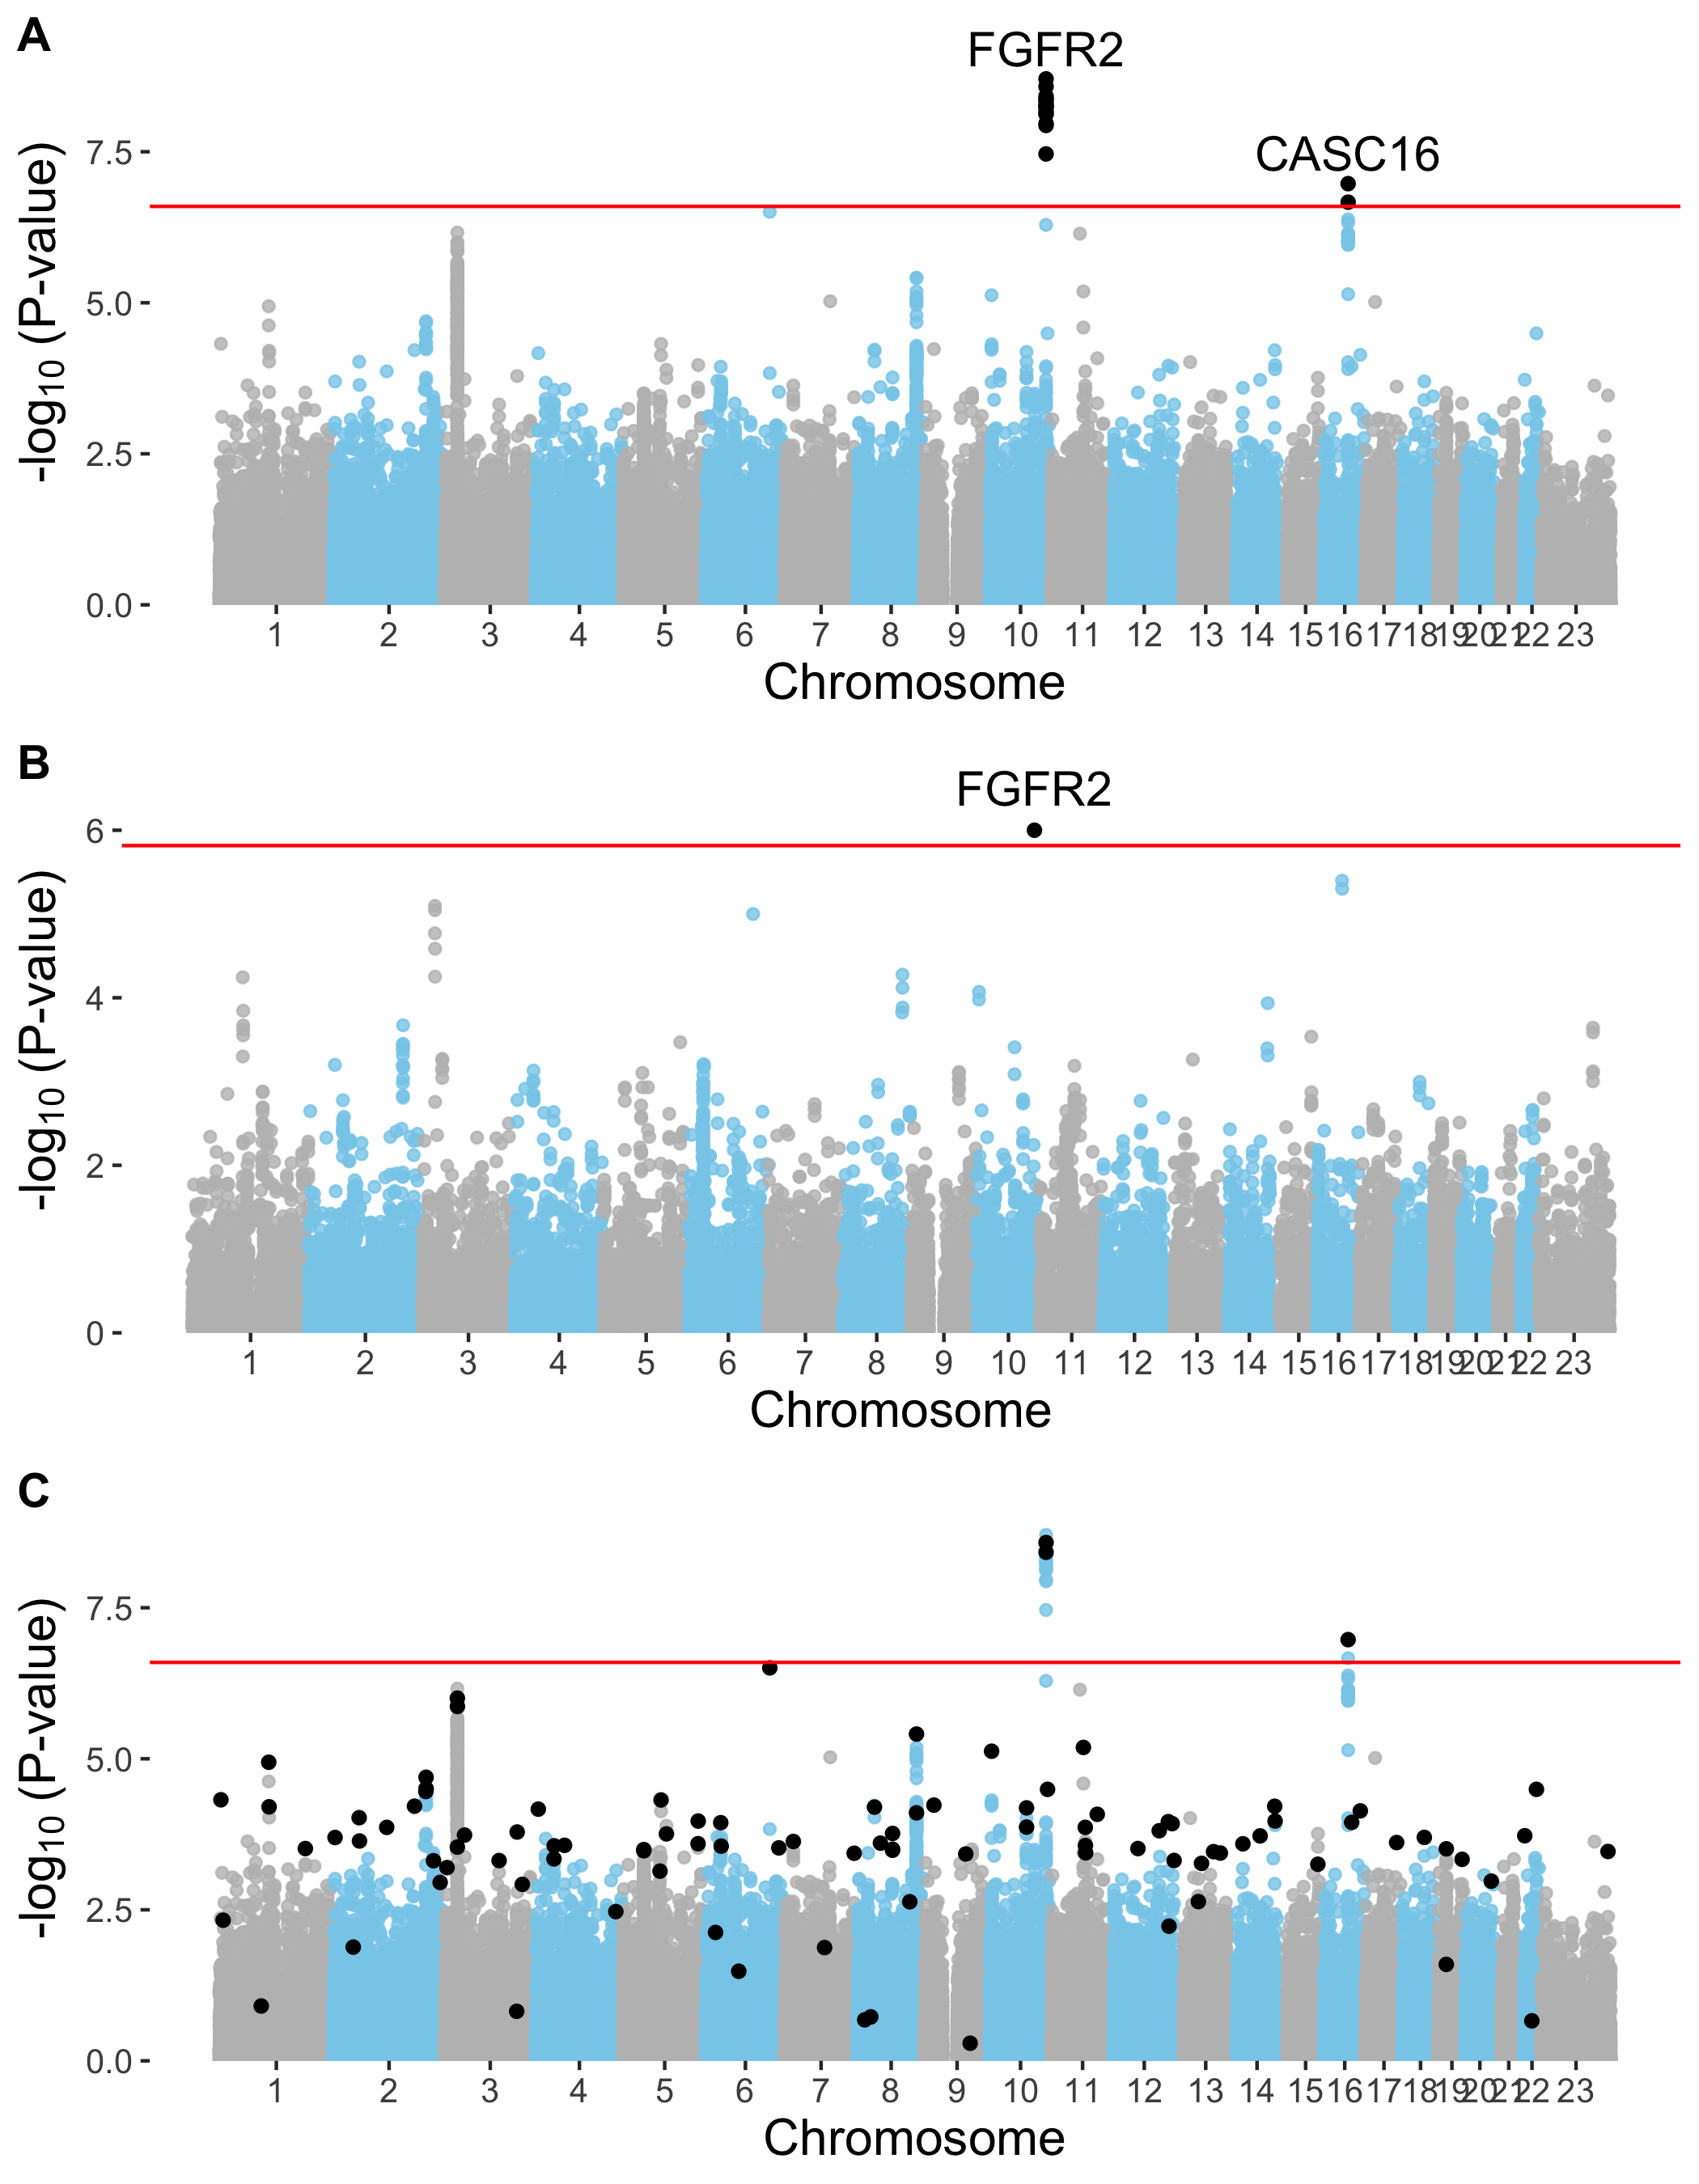
\includegraphics[width=.7\linewidth]{./figures/sfigure_2.png}
  \caption{\label{sfig:snp_gene_manhattan} Association in GENESIS. The red line represents the Bonferroni threshold. \textbf{(A)} SNP association, measured from the outcome of a 1 d.f. $\chi^2$ allelic test. Significant SNPs that are within a coding gene, or within 50 kilobases of its boundaries, are annotated. The Bonferroni threshold is 2.54 \texttimes{} 10\textsuperscript{-7}. \textbf{(B)} Gene association, measured by P-value of VEGAS2v2 \cite{mishra_vegas2:_2015} using the 10\% of SNPs with the lowest P-values. The Bonferroni threshold is 1.53 \texttimes{} 10\textsuperscript{-6}. \textbf{(C)} SNP association as in panel (A). The SNPs in black are selected by a L1-penalized logistic regression (Section~\ref{methods:classifier}, $\lambda = 0.03$).}
\end{figure}

\begin{figure}[htbp]
\centering
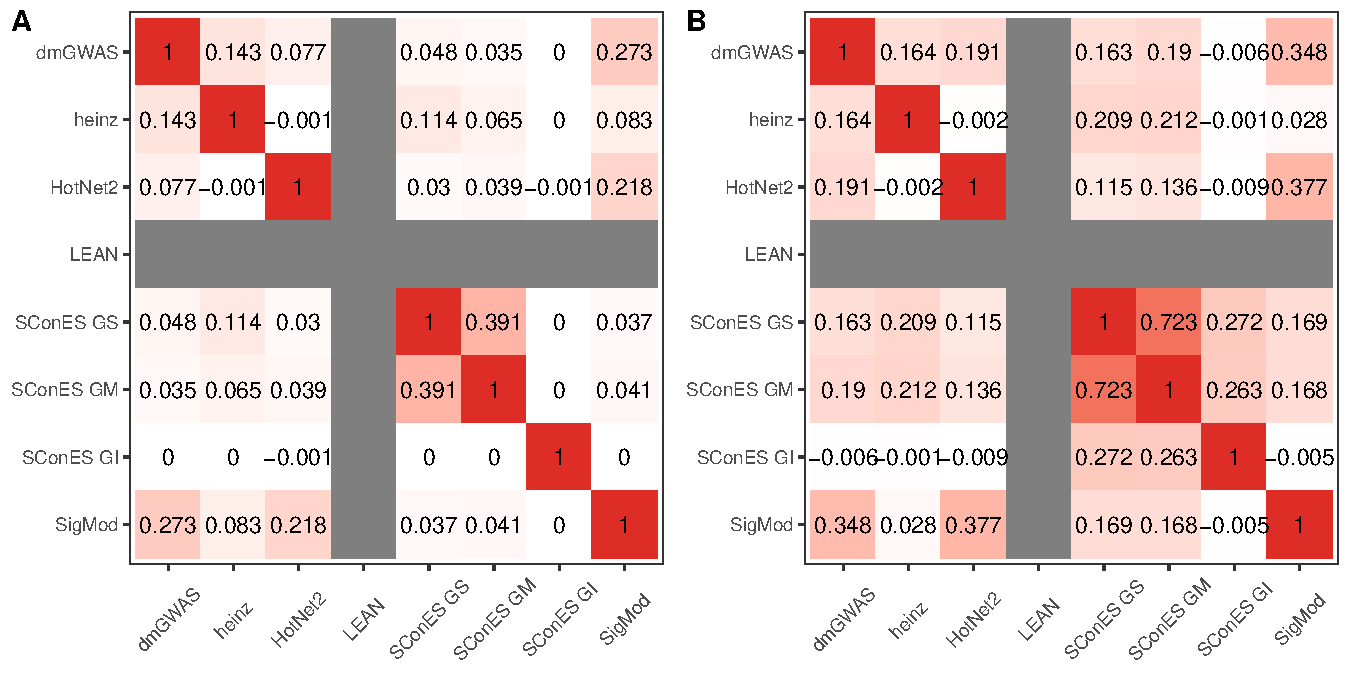
\includegraphics[width=.9\linewidth]{./figures/sfigure_3.pdf}
\caption{\label{sfig:pearson_methods}
Pearson correlation between the different solution subnetworks. \textbf{(A)} Correlation between selected SNPs. \textbf{(B)} Correlation between selected genes. In general, the solutions display a very low overlap.}
\end{figure}

\begin{figure}[htbp]
\centering
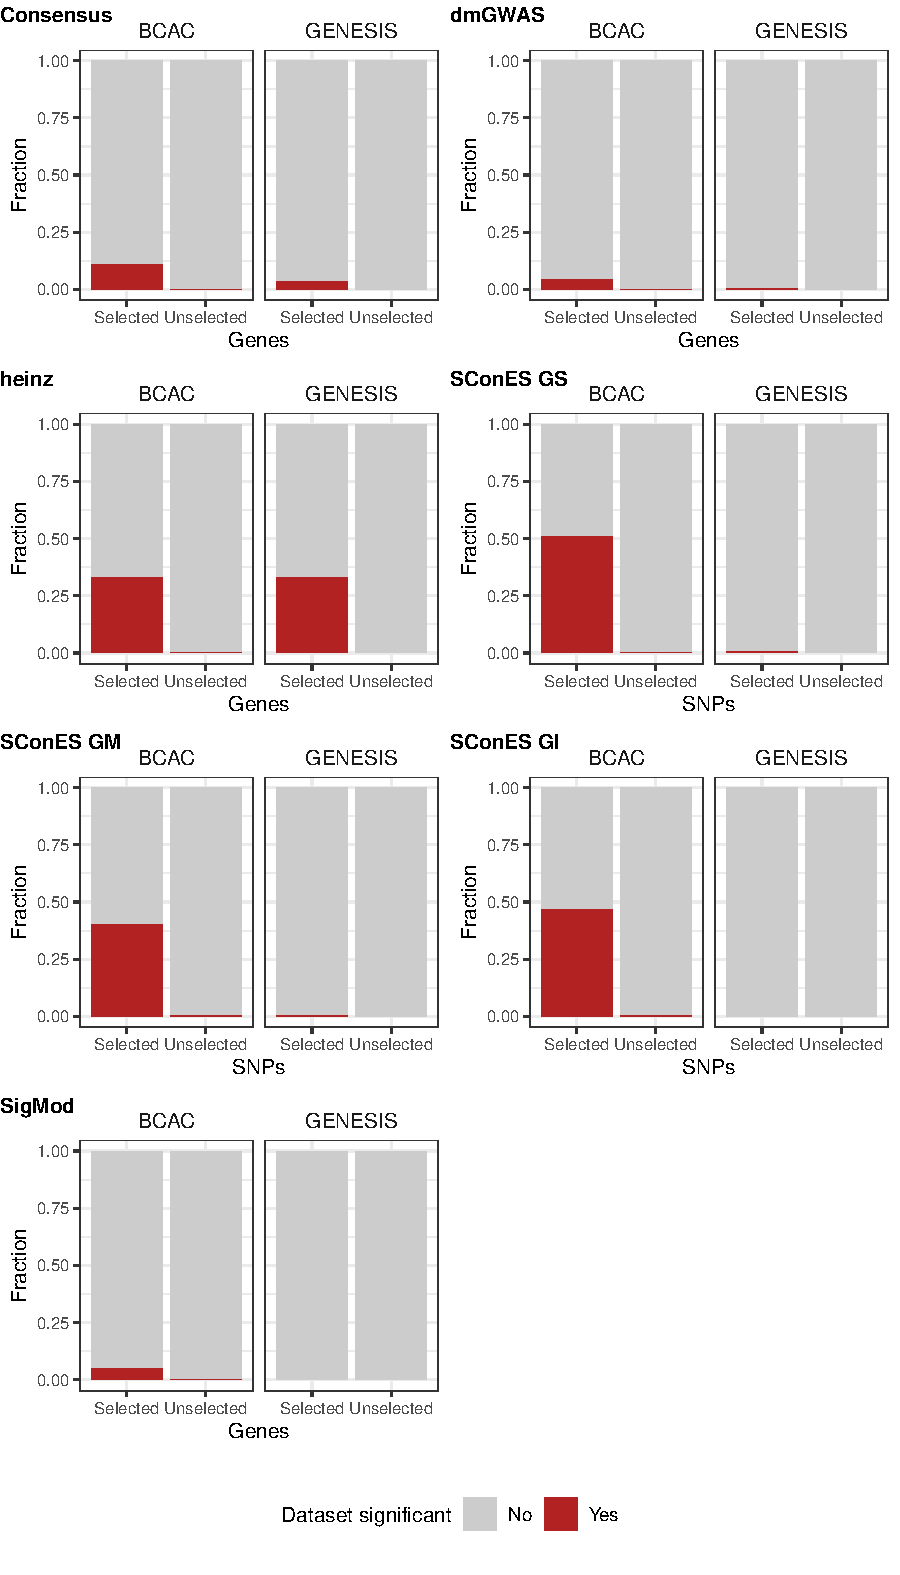
\includegraphics[width=.9\linewidth]{./figures/sfigure_4.pdf}
\caption{\label{sfig:consensus_names}
Consensus subnetwork on GENESIS (Section~\ref{methods:methods}). \textbf{(A)} Each node is represented by a pie chart, which shows the methods that selected it. The labeled genes have a VEGAS2v2 P-value < 0.001 and/or are known breast cancer susceptibility genes (colored in pink). This panel is identical to Figure~\ref{fig:consensus}. \textbf{(B)} Manhattan plot showing the genes included in the subnetwork. \textbf{(C)} Every gene name is indicated. \textbf{(D,E)} Proportion of the Bonferroni significant genes (in GENESIS and BCAC, respectively) included in the consensus network. \textbf{F} Proportion of the selected genes by each of the methods on the GENESIS data that is a known breast cancer susceptibility gene.}
\end{figure}

\begin{figure}[htbp]
\centering
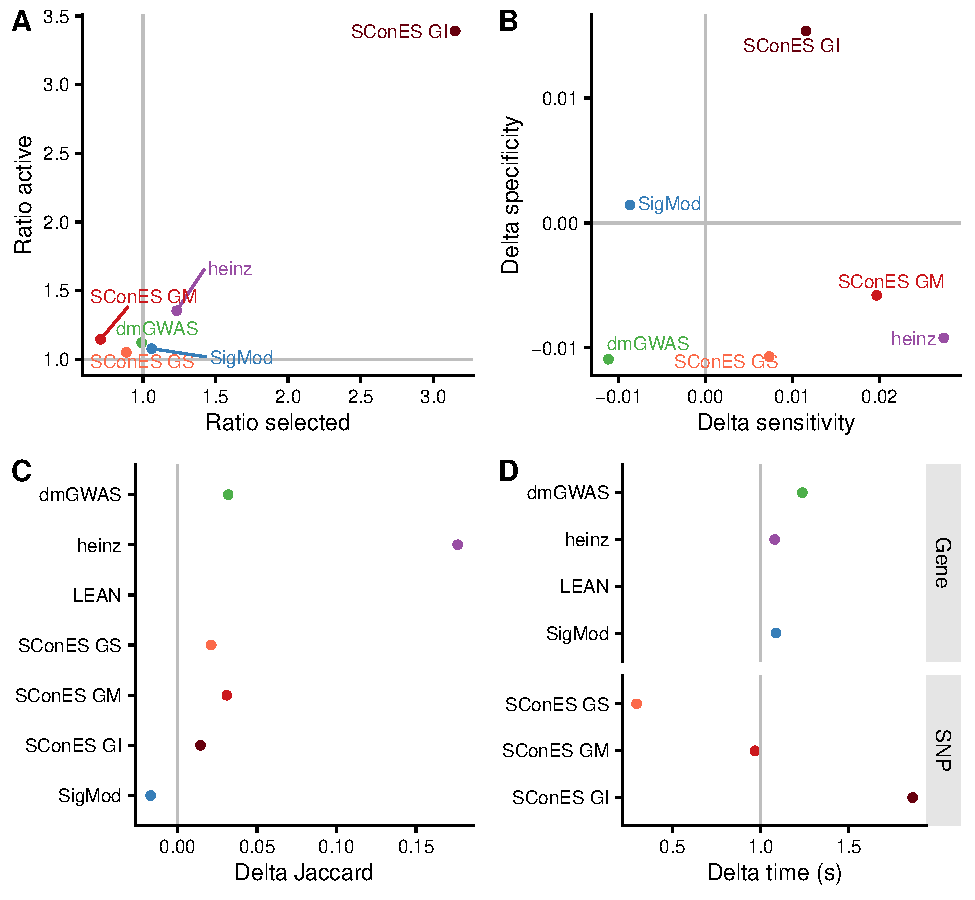
\includegraphics[width=.65\textwidth]{./figures/sfigure_5.pdf}
\caption{\label{sfig:consensus_stats}
Genes on the consensus network. Breast cancer susceptibility genes are colored in pink; the rest are colored in grey. \textbf{(A)} Number of methods selecting every gene in the subnetwork. \textbf{(B)} VEGAS P-values of association of the genes, with regards to the number of methods that selected them. \textbf{(C)} Comparison of betweenness centrality of the genes in the consensus network and the other genes in the PPIN and not in the consensus network. To improve visualization, we removed outliers. \textbf{(D)} Relationship between the log\textsubscript{10} of the betweenness centrality and the -log\textsubscript{10} of the VEGAS P-value of the genes in the consensus network. The blue line represents a fitted generalized linear model.}
\end{figure}

\begin{figure}[htbp]
\centering
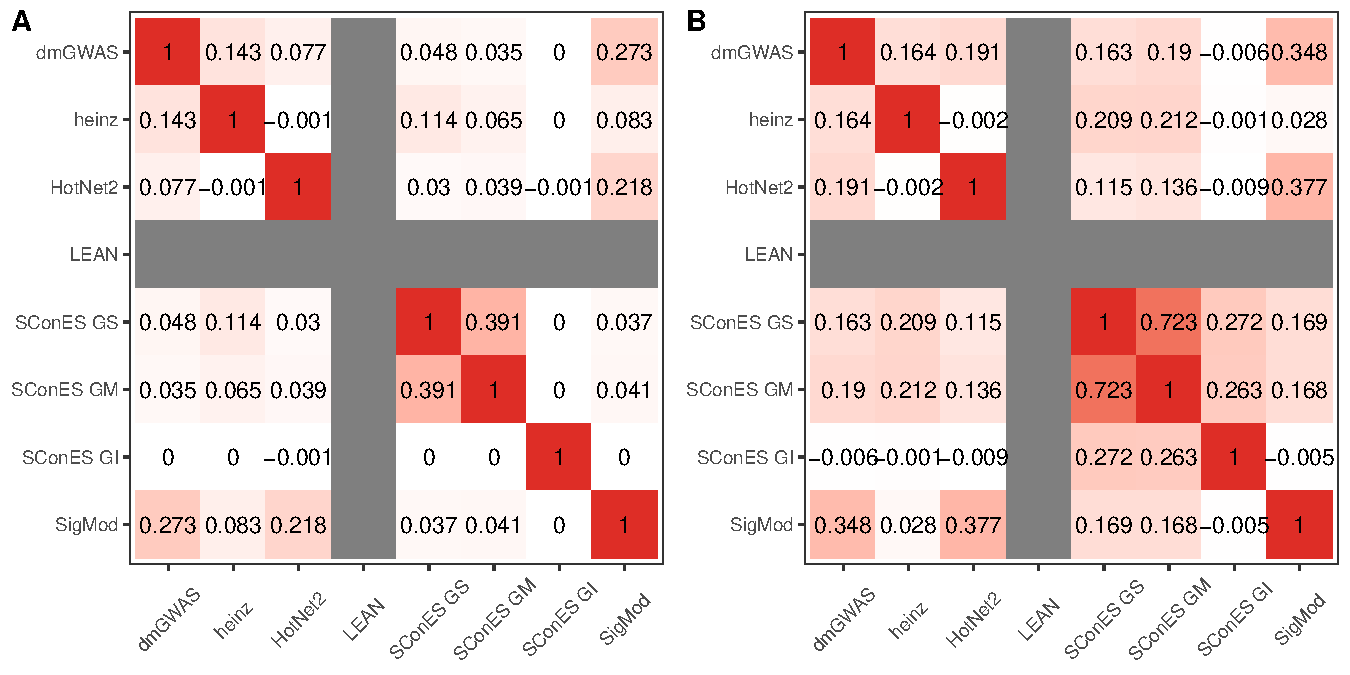
\includegraphics[width=.9\linewidth]{./figures/sfigure_6.pdf}
\caption{\label{sfig:biotypes_excluded}
Biotypes of genes from the annotation that are not present in the HINT protein-protein interaction network.}
\end{figure}

\begin{figure}[htbp]
\centering
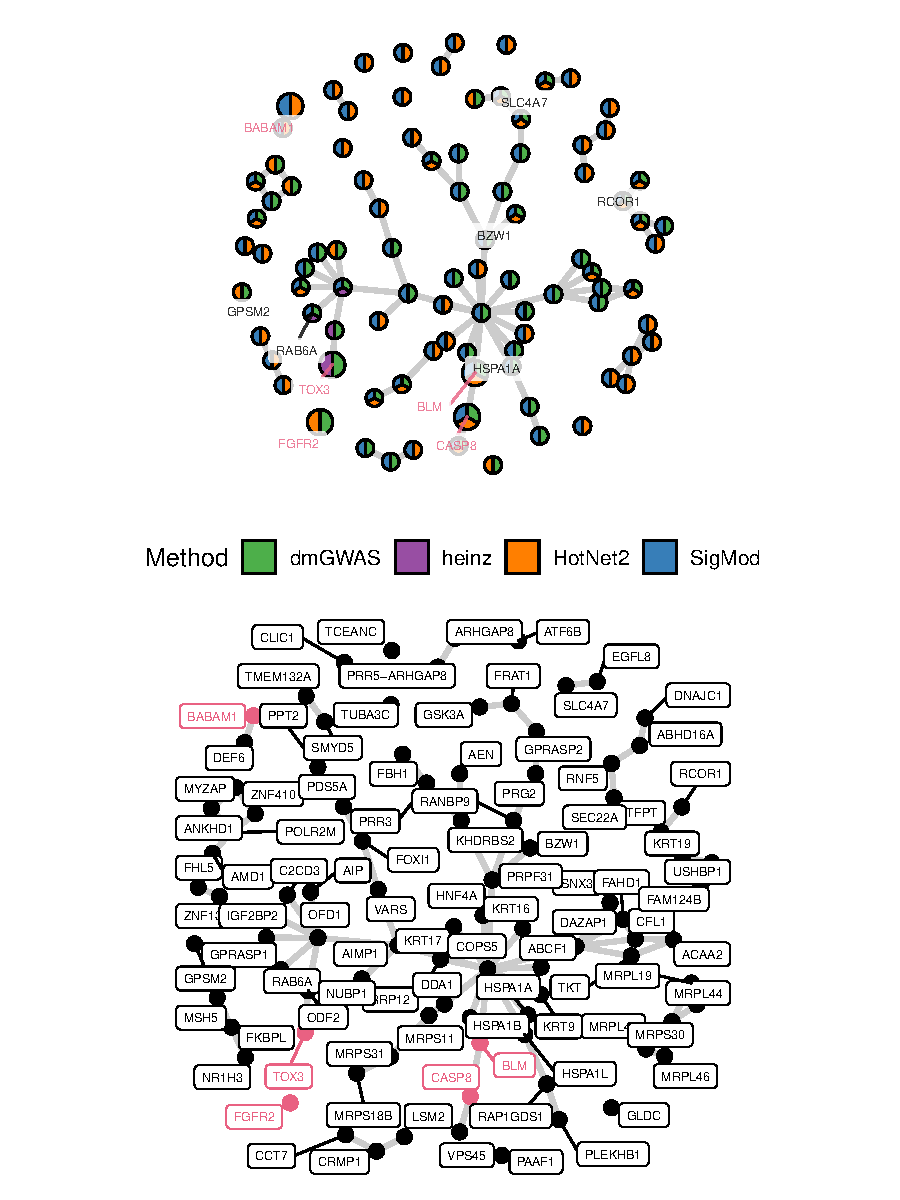
\includegraphics[width=.85\linewidth]{./figures/sfigure_7.pdf}
\caption{\label{sfig:lc_ht_comparison}
Comparison of benchmark on high-throughput interactions to benchmark on both high-throughput and literature curated interactions. Grey lines represent no change between the benchmarks (1 for ratios, 0 for differences). \textbf{(A)} Ratios of the selected features between both benchmarks and of the active set. \textbf{(B)} Shifts in sensitivity and specificity. \textbf{(C)} Shift in Pearson correlation between benchmarks. \textbf{(D)} Ratio between the runtimes of the benchmarks. For gene network-based methods, inverted triangles represent the ratio of runtimes of the algorithms themselves, and circles the total time, which includes the algorithm themselves and the additional 119\,980 seconds (1 day and 9.33 hours) \caz{which took VEGAS2v2}{that VEGAS2v2 took} on average to compute the gene scores from SNP summary statistics. In general, adding additional interactions slightly improves the stability of the solution, but increases the solution size, has mixed effects on the sensitivity and specificity, and impacts negatively the required runtime of the algorithms.}
\end{figure}

\begin{figure}[htbp]
  \centering
  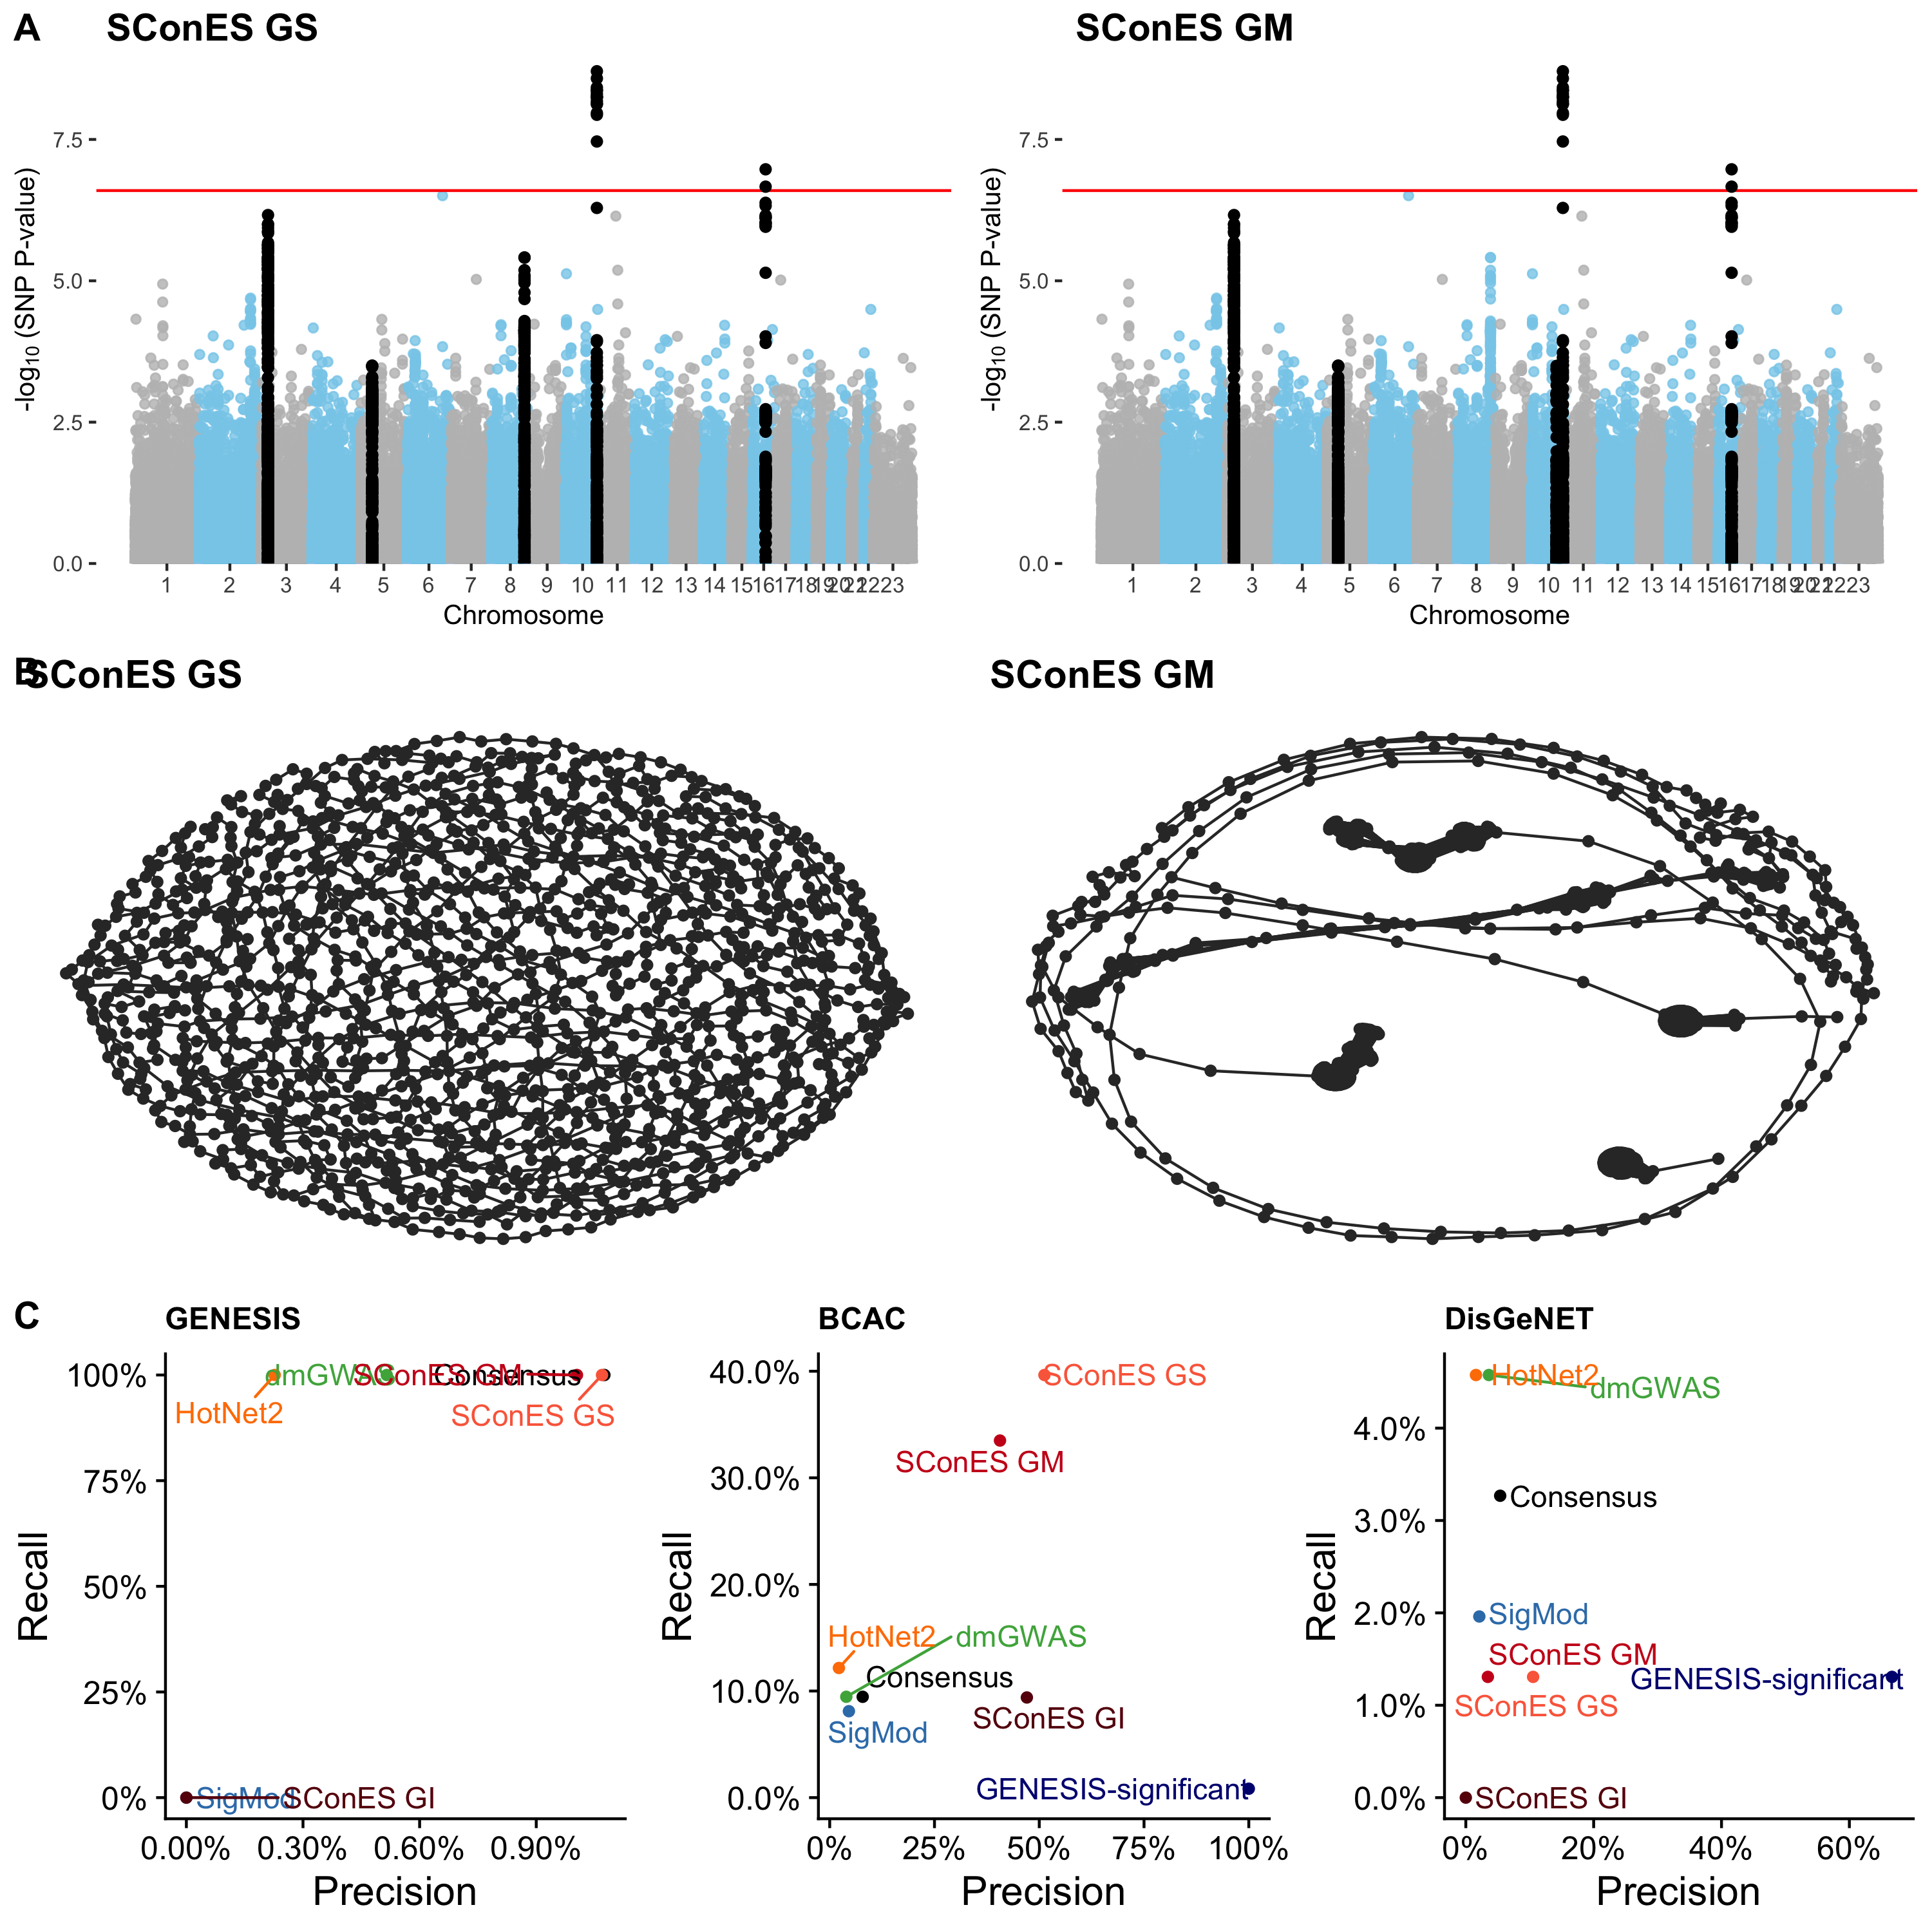
\includegraphics[width=.9\linewidth]{./figures/sfigure_8.png}
  \caption{\label{sfig:scones_gsm} TODO.}
\end{figure}

\end{document}
